\documentclass{article}

\usepackage{graphicx}
\usepackage{subcaption}
\usepackage{float}
\usepackage{hyperref}
\usepackage{amsmath}
\usepackage{amssymb}
\usepackage{enumitem}

\begin{document}

\title{Cross Validation for PCA}
\author{Luca Bulgarelli, Alessandro Ferrera and Vincenzo Sigillò Massara}
\date{}

\maketitle

\begin{abstract}
Principal Component Analysis (PCA) is one of the most widely used multivariate techniques for describing and summarizing data. 
However, determining the optimal number of components remains a critical challenge, particularly in the presence of noisy data. 
While qualitative approaches, such as the scree plot or the percentage of variance explained, are commonly employed, their reliability is often limited. 
In this study, we explore quantitative methods for selecting the optimal number of components, focusing specifically on three cross-validation techniques: 
Gabriel Hold Out, EM-Wold and by Matrix Completion. 
These methods are evaluated through simulations on synthetic datasets and subsequently applied to a real-world dataset to assess their performance and practicality.
Our results suggest that cross-validation techniques can provide a more robust and reliable approach to selecting the optimal number of components in PCA,
compared to traditional qualitative methods, in particular ... .
\end{abstract}

\section{Introduction}
Dimensionality reduction is a fundamental task in data analysis, particularly when dealing with high-dimensional datasets. Its use 
is motivated by the need to simplify the data representation, reduce computational complexity, and improve interpretability. \\
One of the most popular techniques for dimensionality reduction is Principal Component Analysis (PCA), which aims to transform 
the data into a new coordinate system where the variance of the data is maximized along the principal components. Given 
a data matrix $X \in \mathbb{R}^{n \times p}$, PCA seeks to solve the following optimization problem:
\begin{gather*}
    \min_{\hat{X}} \| X - \hat{X} \|_F \quad \text{subject to} \quad \text{rank}(\hat{X}) \leq k 
\end{gather*}
The unsupervised problem can be approached using either the reduced Singular Value Decomposition (SVD) or the eigendecomposition of the covariance matrix. \\
However, a key challenge in PCA is determining the optimal number of components to retain. If too few components are selected, important information may 
be omitted from the analysis. Conversely, retaining too many components can incorporate noise, leading to unstable and unreliable results. \\
Many criteria have been proposed in the literature in order to find the optimal number of dimensions in PCA.
Among the most popular are the scree plot and the percentage of variance explained. \\
The scree plot is a graphical method that displays the eigenvalues of the covariance matrix in decreasing order. The optimal number of components is 
determined by identifying the "elbow" of the curve, where the eigenvalues start to level off. \\
The percentage of variance explained is another common criterion, which selects the number of components that explain a certain percentage of the total variance. 
Typically, a threshold of 80-90\% is used to determine the optimal number of components. \\
While these qualitative approaches are widely used, they are often subjective and lack a rigorous statistical foundation, as a consequence they can bring to
sub-optimal results. \\
Our aim is to explore quantitative methods for selecting the optimal number of components in PCA, focusing specifically on cross-validation techniques.
$\\ \\$
The report is organized as follows. \textbf{Section 2} is dedicated to the illustration of methods implemented in the study, and their theoretical background.
\textbf{Section 3} describes the creation of synthetic datasets and the real dataset used. \textbf{Section 4} presents the results of the simulations and the 
application of the methods to the real dataset. Finally, \textbf{Section 5} concludes the report.

\section{Methodology}
In this section, we outline the cross-validation techniques employed to determine the optimal number of components in PCA. \\ \\
The primary challenge in cross-validation lies in balancing the trade-off between bias and variance. However, in the unsupervised setting of PCA,  
a straightforward approach to cross-validation is not suitable. Specifically, splitting the data into training and test sets, then evaluating model performance 
to select the number of components that minimizes the error, would yield misleading results. This approach would consistently favor the maximum number of components, 
as a larger subspace always fits the data points more effectively. The absence of a proper bias-variance trade-off in this context inevitably leads to overfitting. \\  
To address this issue, we consider three cross-validation techniques that are specifically tailored to PCA:
\begin{enumerate}[label=(\alph*)] 
    \item Gabriel Hold Out Cross Validation
    \item Cross Validation with EM
    \item Cross Validation by Matrix Completion
\end{enumerate}
We now provide a brief overview of each method.

\subsection{Gabriel Hold Out Cross Validation}
The first method aims to transform PCA from an unsupervised problem to a supervised one, with a sensible approach that can capture some bias-variance trade-off. In particular, this method assumes that the data matrix \textbf{X} is composed of i.i.d. observations of a multivariate Gaussian distribution with mean $\mu \in \mathbb{R}^p$ and covariance matrix $\Sigma \in \mathbb{R}^{p \times p}$. We partition the observations in K-folds and, for every possible rank $R = 1, ..., p$, we operate as follow on each fold $E^k$:
\begin{itemize}
	\item We estimate $\mu$ and $\Sigma$ from the observations that are not in the fold $E^k$ with sample mean and covariance estimators $\hat{\mu}$ and $\hat{\Sigma}$. 
	\item We perform the spectral truncation of the covariance matrix $\Sigma$ to retain only the first $R$ eigenvalues.
          Given the eigendecomposition of the covariance matrix: $\Sigma = U \Lambda U^\top$, we let $\tilde{\Lambda}$ be 
          the diagonal matrix obtained by setting to zero all but the $R$ largest eigenvalues of $\Sigma$, and we pose
          $\tilde{\Sigma} = U \tilde{\Lambda} U^\top$.
          \item Each observation in $E^k$ is randomly split into two parts: $\textbf{x}^{miss}$ (a proportion $\pi$ of the features) and $\textbf{x}^{obs}$ (the remaining 1 - $\pi$)  that will be considered respectively as the missing and observed part in the following steps
	\item With the assumption of Gaussianity, assuming we can write the $i$-th observation as follows:
	$$
	\textbf{x}^{(i)} = \begin{bmatrix} \textbf{x}^{(i)}_\text{obs} \\ \textbf{x}^{(i)}_\text{miss} \end{bmatrix} \quad
                \mu = \begin{bmatrix} \mu_\text{obs} \\ \mu_\text{miss} \end{bmatrix} \quad
                \tilde{\Sigma} = \begin{bmatrix} \tilde{\Sigma}_{\text{obs}} & \tilde{\Sigma}_\text{miss,obs} \\ \tilde{\Sigma}_\text{obs,miss} & \Sigma_{\text{miss}} \end{bmatrix}
	$$
	we can estimate the missing part with its conditional expectation  as follows 
	\begin{equation}
	\hat{\textbf{x}}^{(i)}_\text{miss} = \mathbb{E}_{\mu,\tilde{\Sigma}} \left[ \textbf{x}^{(i)}_\text{miss} | \textbf{x}^{(i)}_\text{obs} \right] = \mu_\text{miss} + \tilde{\Sigma}_{\text{miss,obs}} \tilde{\Sigma}_{\text{obs}}^{\dag} \left( \textbf{x}^{(i)}_\text{obs} - \mu_\text{obs} \right)
	\label{eq:condexp}
	\end{equation}
	where $\dag$  indicates Moore-Penrose pseudoinverse.
	\item Finally, we can compute the error for the $k$-th fold as 
	$$
	\text{err}^k = \frac{1}{\pi p|E^k|}\sum_{i \in E^k} \| \hat{\textbf{x}}^{(i)}_\text{miss} - \textbf{x}^{(i)}_\text{miss} \|_2^2
	$$
	to ensure consistency with the errors calculated with the other methods.
\end{itemize}
Once we computed the error on each fold, we average them to obtain the cross-validation error for rank $R$.

\subsection{Cross Validation with EM}
This method builds upon the same idea as the previous approach but incorporates the Expectation-Maximization (EM) Algorithm. 
As before, we use the assuwqmption that the data matrix is generated from a Gaussian distribution. \\ 
Given a data matrix $X \in \mathbb{R}^{n \times p}$, with rows defined as before, we can proceed as follows.  
Fixed the number \( R \) of principal components to retain, we partition the entries of the data matrix into 
$K$ folds $E^k$ for $k = 1, 2, \dots, K$. For each fold, we repeat the following steps:
\begin{itemize}
    \item On the matrix $X$ with the entries of the fold $E^k$ set to missing, we use EM to estimate the parameters of 
          the Gaussian distribution: $\mu$ and $\Sigma$.
    \item We perform the spectral truncation of the covariance matrix $\Sigma$ as in the previous method.
    \item For every row $i$ of the data matrix, we predict the missing entries as the conditional expectation of the
          unobserved entries given the observed ones, i.e. $\hat{\textbf{x}}^{(i)}_\text{miss} = \mathbb{E}_{\mu,\tilde{\Sigma}}
          \left[ \textbf{x}^{(i)}_\text{miss} | \textbf{x}^{(i)}_\text{obs} \right]$ for $i = 1, 2, \dots, n$. 
          Assuming that the data is Gaussian, we can perform the estimation using \eqref{eq:condexp}.
     \item  As a result, we can compute the error for the fold $E^k$ as:
            \begin{gather*}
                \text{err}^k = \frac{1}{|E^k|} \sum_{(i,j) \in E^k} (X_{ij} - \hat{X}_{ij})^2
            \end{gather*}
         Instead, if the i-th row of the data matrix is completely observed, the error is null.
\end{itemize}    
In the end, we average the errors to obtain the cross-validation error for rank $R$.\\

\subsection{Cross Validation by Matrix Completion}
This method exploits the problem of the Matrix Completion, which consists in estimating the missing entries of a matrix given the observed ones. In our setting,
we are considering a problem of low-rank Matrix Completion. \\
In particular, given a data matrix $X \in \mathbb{R}^{n \times p}$ and a bivariate index set $\Omega$, that indicates the observed entries of $X$,
the problem of matrix completion is equivalent to the following optimization problem with rank constraint:
\begin{gather*}
    \underset{M}{\text{argmin}} \sum_{(i,j) \in \Omega} (X_{ij} - M_{ij})^2 \quad \text{subject to} \quad \text{rank}(M) = R
\end{gather*}
This problem can be solved using an iterative hard-thresholding algorithm, which updates at each step the approximation via SVD. The method is based on the 
following steps.\\ \\
Let's begin by defining $\tilde{M}^{(0)}$ = $X$ with missing entries. Then for each $l = 1,$ $2, \dots$, we iterate:
\begin{itemize}
    \item We compute the SVD of $\tilde{M}^{(l-1)} = U D V^\top$.
    \item We let $\tilde{D}$ be the diagonal matrix obtained by setting to zero all but the $R$ largest singular values of $D$.
    \item We pose ${M}^{(l)} = U \tilde{D} V^\top$, that has indeed rank $R$. This is our new approximation.
    \item We update, then, $\tilde{M}^{(l)}$ as follows:
    \begin{gather*}
        \tilde{M}^{(l)} = \begin{cases} 
        X_{ij} & \text{if } (i,j) \in \Omega \\
        M^{(l)}_{ij} & \text{otherwise}
        \end{cases}
    \end{gather*}
    \item We evaluate the expression that we aim to minimize:
    \begin{gather*}
        \sum_{(i,j) \in \Omega} (X_{ij} - M^{(l)}_{ij})^2
    \end{gather*}
        If the difference of this quantity between two consecutive approximations is below a certain threshold, we stop the iterations.
\end{itemize}
$\\$
We can use this method to calculate the cross-validation error for different values of $R$. 
\\In particular, we can split the data matrix entries into $K$ folds $E^k$ with $k=1, 2, \dots ,K$, 
and for each, using the previous algorithm, we compute the 
approximation of the matrix $M^k$ with rank $R$ taking as observations the other $K-1$ folds.\\
Then, we evaluate the error on the fold that we left out, so we will have:
\begin{gather*}
    \text{err}^k = \frac{1}{|E^k|} \sum_{(i,j) \in E^k} (X_{ij} - M^k_{ij})^2
\end{gather*}
We repeat this process for all the $K$ folds, and we average the errors to obtain the cross-validation error for rank $R$.\\
Let's remark that this is the only approach in which we are not supposing anything on the distribution of the data.

\section{Datasets for comparison of the methods}
To assess and analyze the performance of the three approaches described above, 
we will utilize simulated data matrices with a dimensionality a-priori known and a real-world dataset.

\subsection{Simulated data}
Normally, the information of the number of components to retain in PCA is not available in real-world datasets, but, since we have to compare the methods in a 
controlled environment, we will generate synthetic data with a known number of components. 
The method to generate the data is taken from \cite{perry}. 
\\
Fixed the number of components $k$, the sample size $n$ and the number of features $p$, we generate the data matrix $X$ as follows:
\begin{itemize}
    \item We generate a matrix $U \in \mathbb{R}^{n \times k}$ with entries $U_{ij} \sim \mathcal{N}\left(0,\frac{1}{n}\right)$
    \item We generate a matrix $V \in \mathbb{R}^{p \times k}$ with entries $V_{ij} \sim \mathcal{N}\left(0,\frac{1}{p}\right)$
    \item We generate the vector of singolar values $d \in \mathbb{R}^k$, accurately choosing
          the range of the entries.
    \item We compute the data matrix $\hat{X} = UDV^\top$
    \item We add noise to the data matrix to obtain the final data matrix.: \\ $X = \hat{X} + E$. 
    The noise will be of three differert types: 
    \begin{enumerate}[label=\alph*.] 
            \item Gaussian: this noise is randomly generated from a standard gaussian distribution $E_{ij} \sim \mathcal{N} (0,1)$
            \item Heavy: this type of noise comes from a Student's t-distribution with $\nu = 3$ degrees of freedom, rescaled over its standard deviation $\sigma = \sqrt{\nu/(\nu - 2)} $
            \item Colored: to simulate heteroscedasticity, we generated $\sigma_1^2,...,\sigma_n^2 \sim \text{Inverse-}\chi ^2(3)$ and $\tau_1^2,...,\tau_p^2 \sim \text{Inverse-}\chi ^2(3)$. Using these values we generated $E_{ij} \sim \mathcal{N} (0,\sigma_i^2 + \tau_j^2)$
    \end{enumerate}
\end{itemize}

\subsection{Real data}
To evaluate the methods in a practical context, we tested them on 
real-world datasets. 
From the literature, we identified a dataset (hereafter referred to as the Aphids dataset) consisting 
of 19 variables measured on 40 winged aphids (\textit{alate adelges}) captured using a 
light trap. \\
The issue of determining the appropriate number of components to retain in PCA for this dataset 
has been previously studied by both Jeffers (1967) \cite{Jeffers} and Krzanowski (1987) \cite{Krzanowski}. 
From \cite{Dray} another dataset emerged, whose intrinsic dimensionality had already been estimated. The
data was comprised of 60 observations of 16 variables regarding air pollution in various areas of the United States.
In both cases, the data was standardized before applying the methods. Moreover, following the steps of \cite{Dray},
some variables ($HC$,$NO_x$ and $SO_2$) were log-transformed.

\section{Results}

We now present the results of the simulations conducted on synthetic datasets, which were designed to thoroughly 
evaluate the performance of the three methods under various conditions. These simulations focused on comparing the 
methods in terms of both performance and runtime, providing valuable insights into their respective strengths and weaknesses. 
In particular, we assessed how each method performed across different scenarios, considering factors such as the complexity of 
the data and the computational resources required.\\
A preliminary step in the analysis was to evaluate the impact of the parameter $\pi$ on the Gabriel Cross-Validation method.\\
Moreover, we paid special attention to the impact of the true rank of the data matrix, as this is a critical factor in determining 
the effectiveness of the methods. By systematically varying the rank, we were able to observe how the methods handled different levels 
of data complexity. Additionally, we explored the influence of sample size, testing how each method performed with varying amounts of data. 
This allowed us to examine whether any of the methods were particularly sensitive to changes in sample size.\\
After addressing these important research questions and drawing conclusions from the synthetic data simulations, 
we proceeded to validate our findings by applying the methods to a real-world dataset. This step allowed us to assess 
how well the methods generalize to practical, real-world scenarios and further confirm the insights gained from the synthetic simulations. 
The validation on real data serves as an important final check to ensure the robustness and applicability of the proposed methods in real-world applications.

\subsection{Discussion of the results on simulated data} 

For our simulations, we created synthetic datasets with varying dimensions 
and levels of noise. In most cases, we manipulated the singular values to obtain 
a data matrix that was more or less perturbed. To assess the effect of the noise 
on the data matrix, we calculated the Signal to Noise Ratio (SNR) as follows:
\begin{gather*}
    \text{SNR} = \frac{\|\hat{X}\|_F}{\|E\|_F}
\end{gather*}
where with $\| \cdot \|_F $ we indicate the Frobenius norm. Moreover, $\hat{X}$ is the data matrix without noise and $E$ is the noise matrix.

\subsubsection{Choice of hyperparameter of Gabriel CV}
The first aspect we analyzed was the impact of the parameter $\pi$ on the Gabriel CV. In fact, the choice of this parameter
is crucial for the performance of the method. In Figure \ref{fig:gabriel_pi}, we tested the algorithm for three values of $\pi = 0.6 , 0.7, 0.8$, 
fixing the true rank of the data matrix to $5$. We also run the algorithm for the different type of noise. \\
As we can see from the plots, 
a high value of $\pi$ yields an uncertain behaviour: the correct true size is in fact chosen by the method but not with a significant 
difference from the neighbouring sizes. A lower value of $\pi$, on the other hand, denotes a more convinced selection of the true size but also 
a more unstable behaviour for a large number of components. A value between $0.6$ and $0.7$ seems to be a sensible choice.
In this simulation we fixed the sample size to $1000$ and the number of features to $30$. We tried the same experiment with different values of $n$
and the results were consistent with the ones shown in the figure.
\begin{figure}[h!]
    \centering
    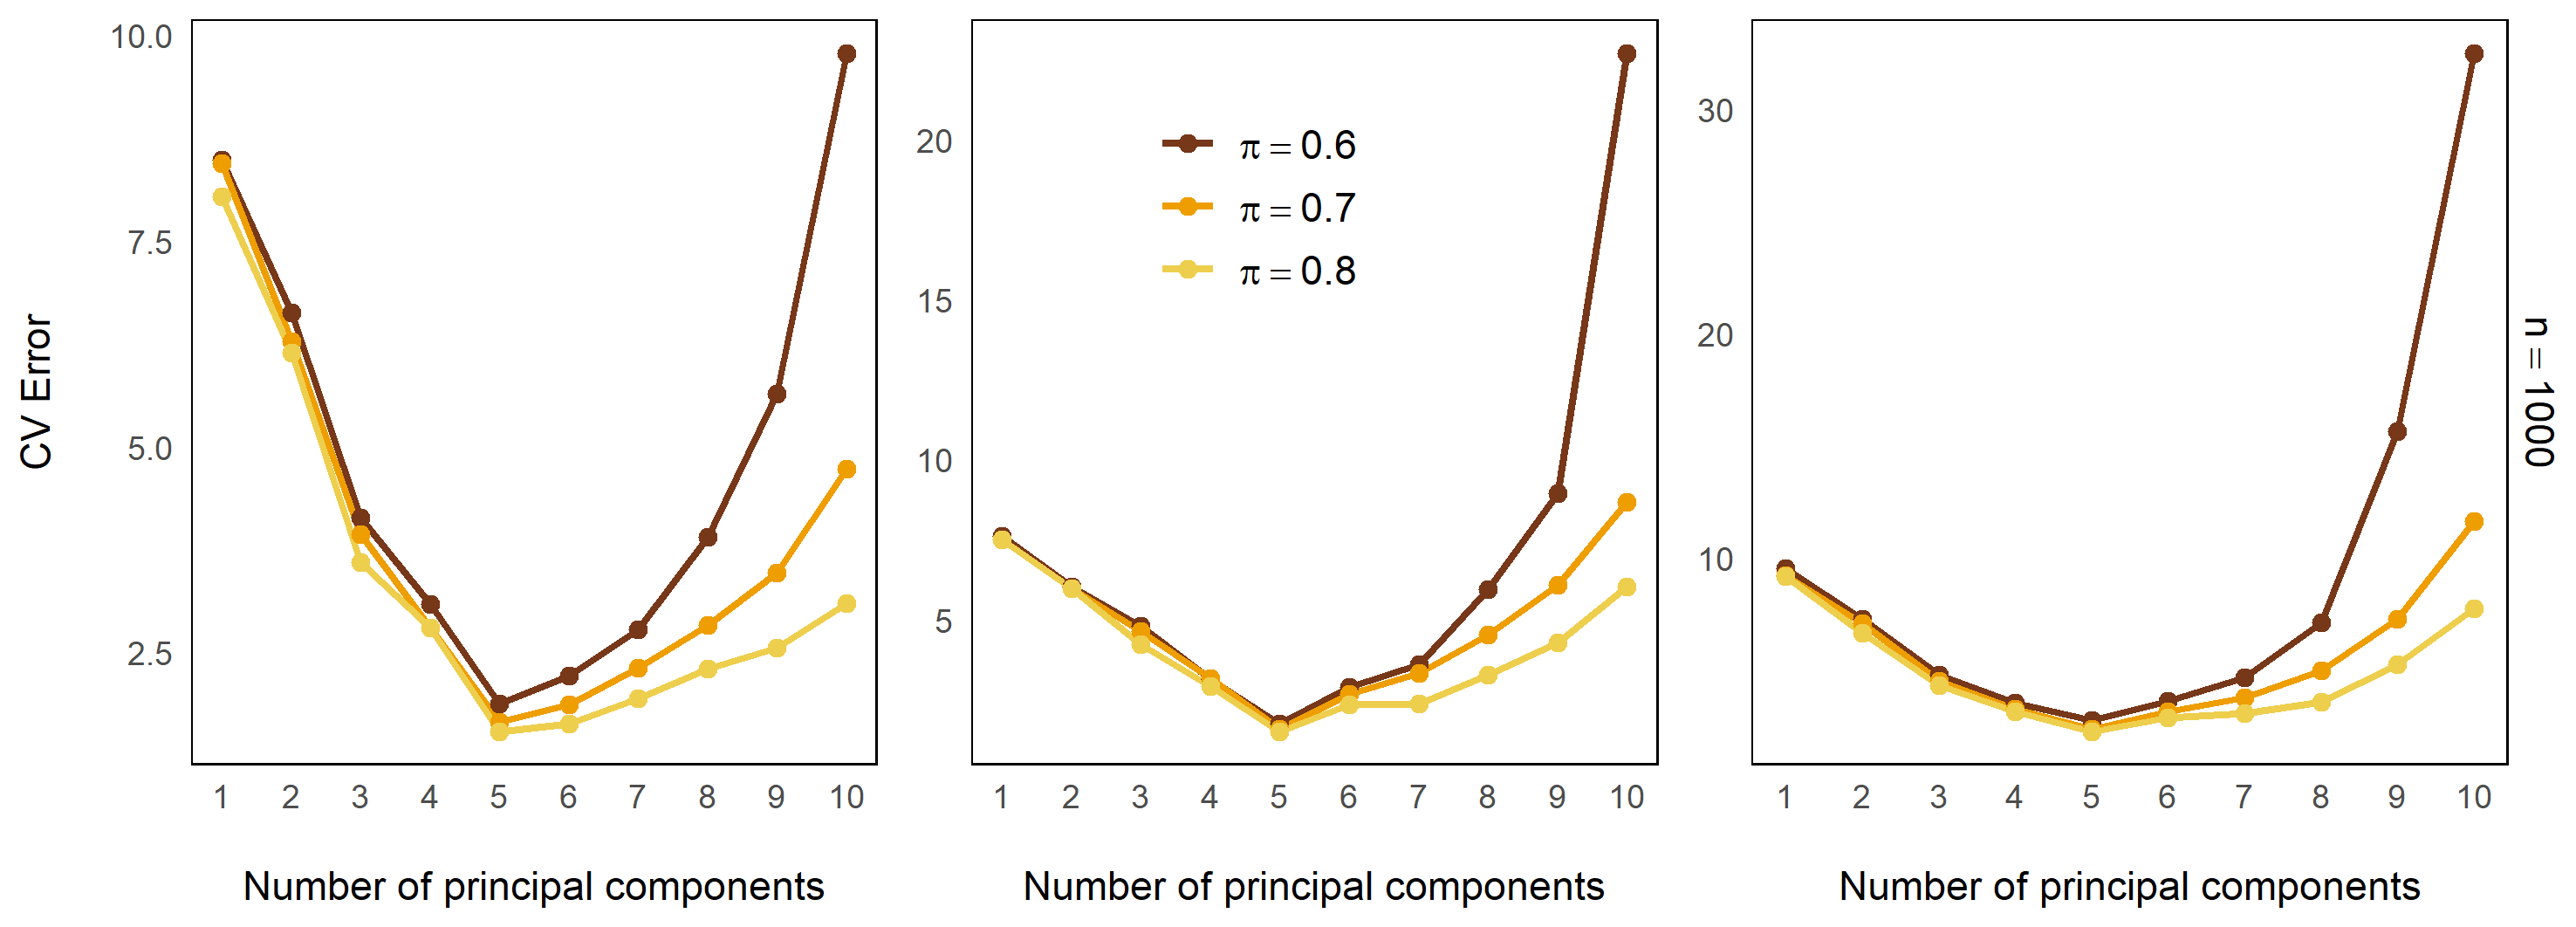
\includegraphics[width=0.95\textwidth]{Gabriel.png}
    \caption{Impact of $\pi$ on Gabriel CV}
    \label{fig:gabriel_pi}
\end{figure}

\subsubsection{Comparison of the methods}
As a first term of comparison, we analysed the error plots of the three 
methods with the three types of noise described in section 3.1, with fixed 
parameters $n=1000, p=30$, true rank $R = 5$ on a 10-fold cross-validation. 
We will keep this setting also for the following simulations, unless specified. \\
As shown in Figure \ref{fig:CV_error}, though all methods seem to yield the 
correct answer, the Matrix Completion algorithm actually remarks the choice 
more strongly, with all three noises. The SNR in this simulation is set high 
($\approx 6$), so the noise is not very impactful on the data matrix.
\begin{figure}[h!]
    \centering
    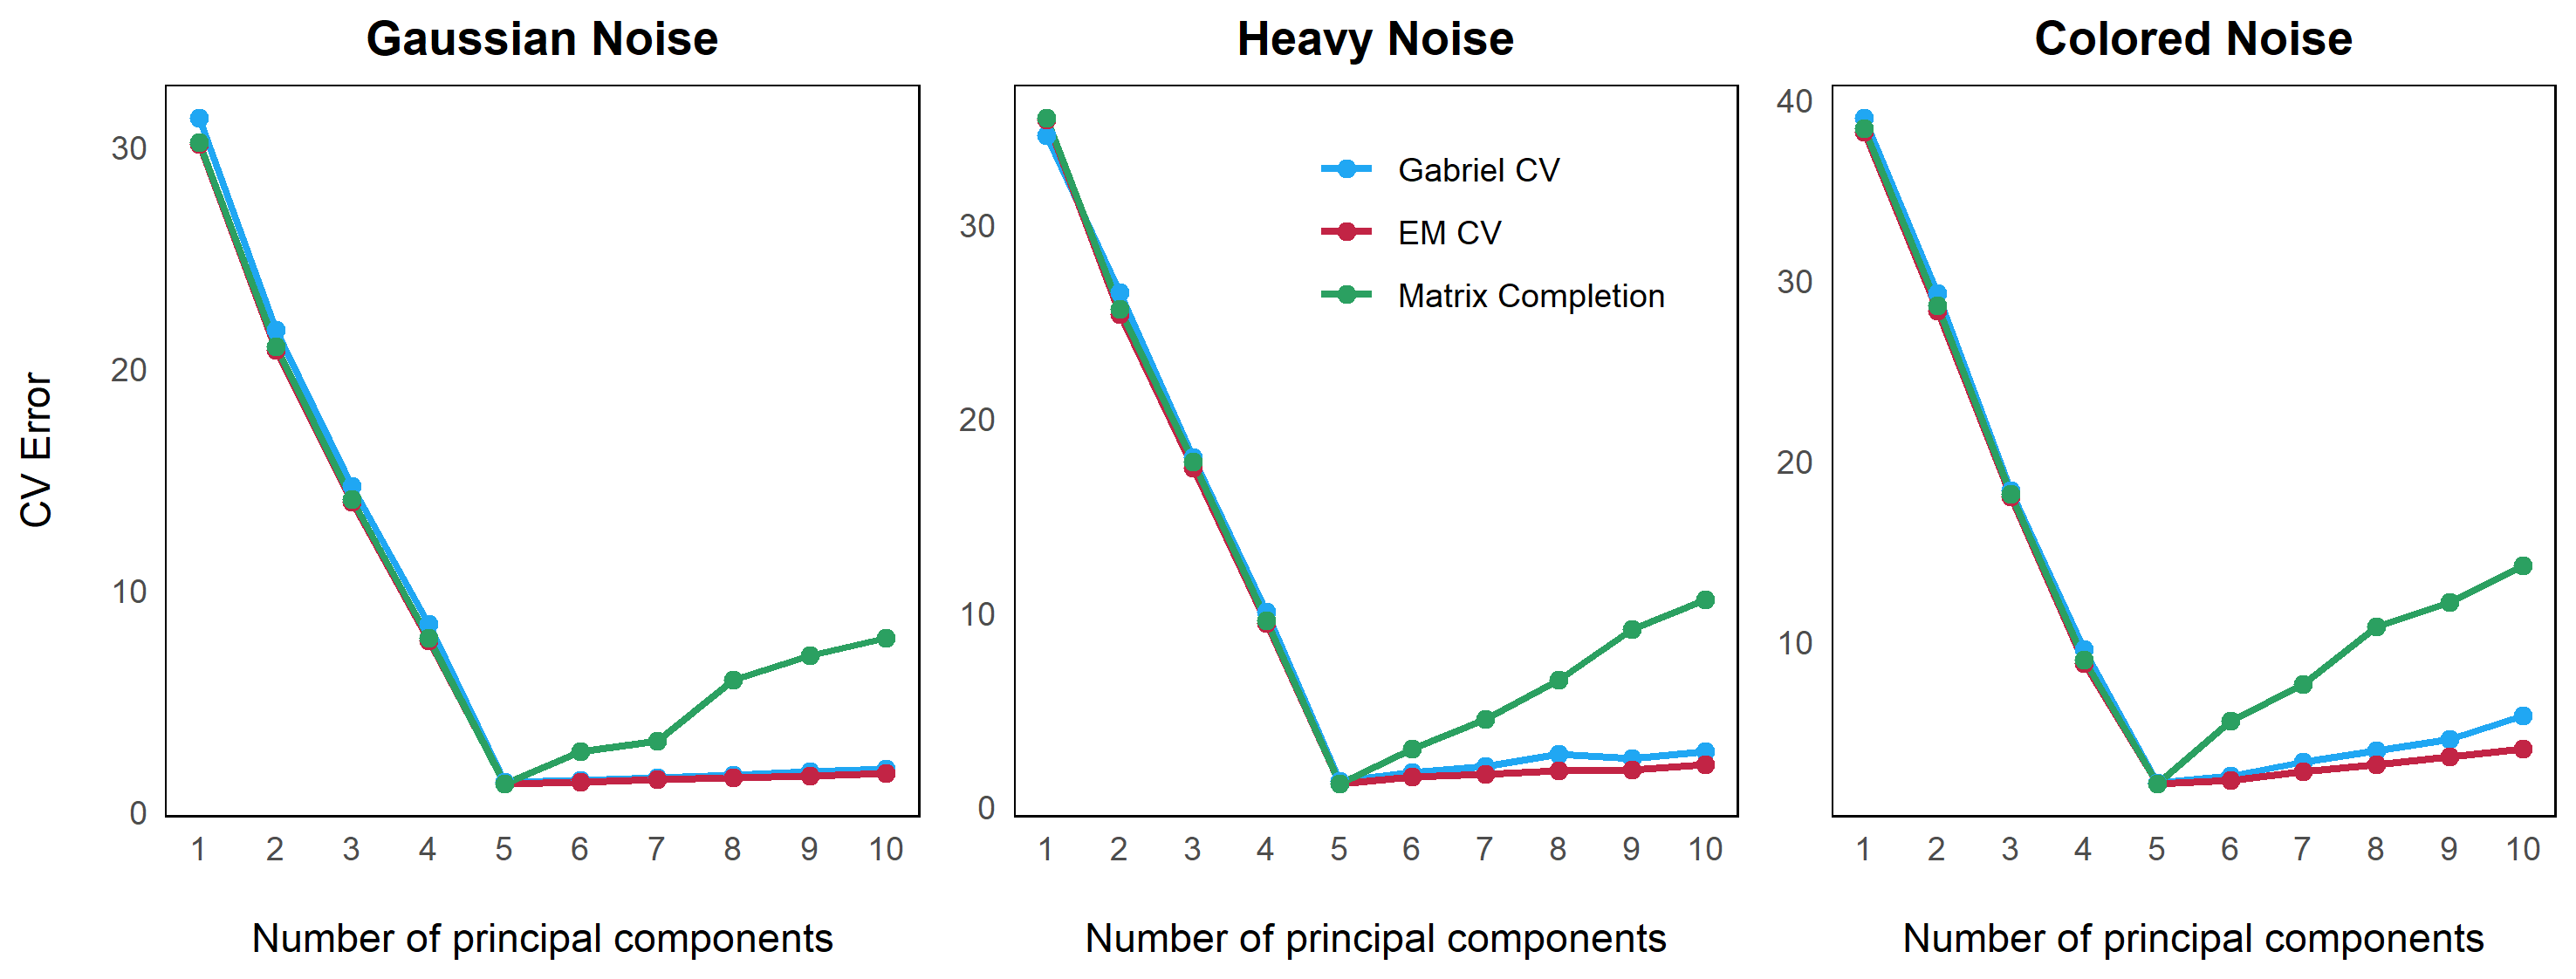
\includegraphics[width=0.95\textwidth]{CVplots.png}
    \caption{CV error of the three methods varying the noise, with high SNR}
    \label{fig:CV_error}
\end{figure}
With a higher noise (lower SNR $\approx 1.5$), all three methods seem to choose the correct non-trivial size more confidently,
as shown in Figure \ref{fig:CV_error_high}. Both the matrix completion and the Gabriel hold-out appear to show
some kind of erratic behaviour when evaluating the error for higher sizes, with the EM cross-validation being 
the most stable.

\begin{figure}[h!]
    \centering
    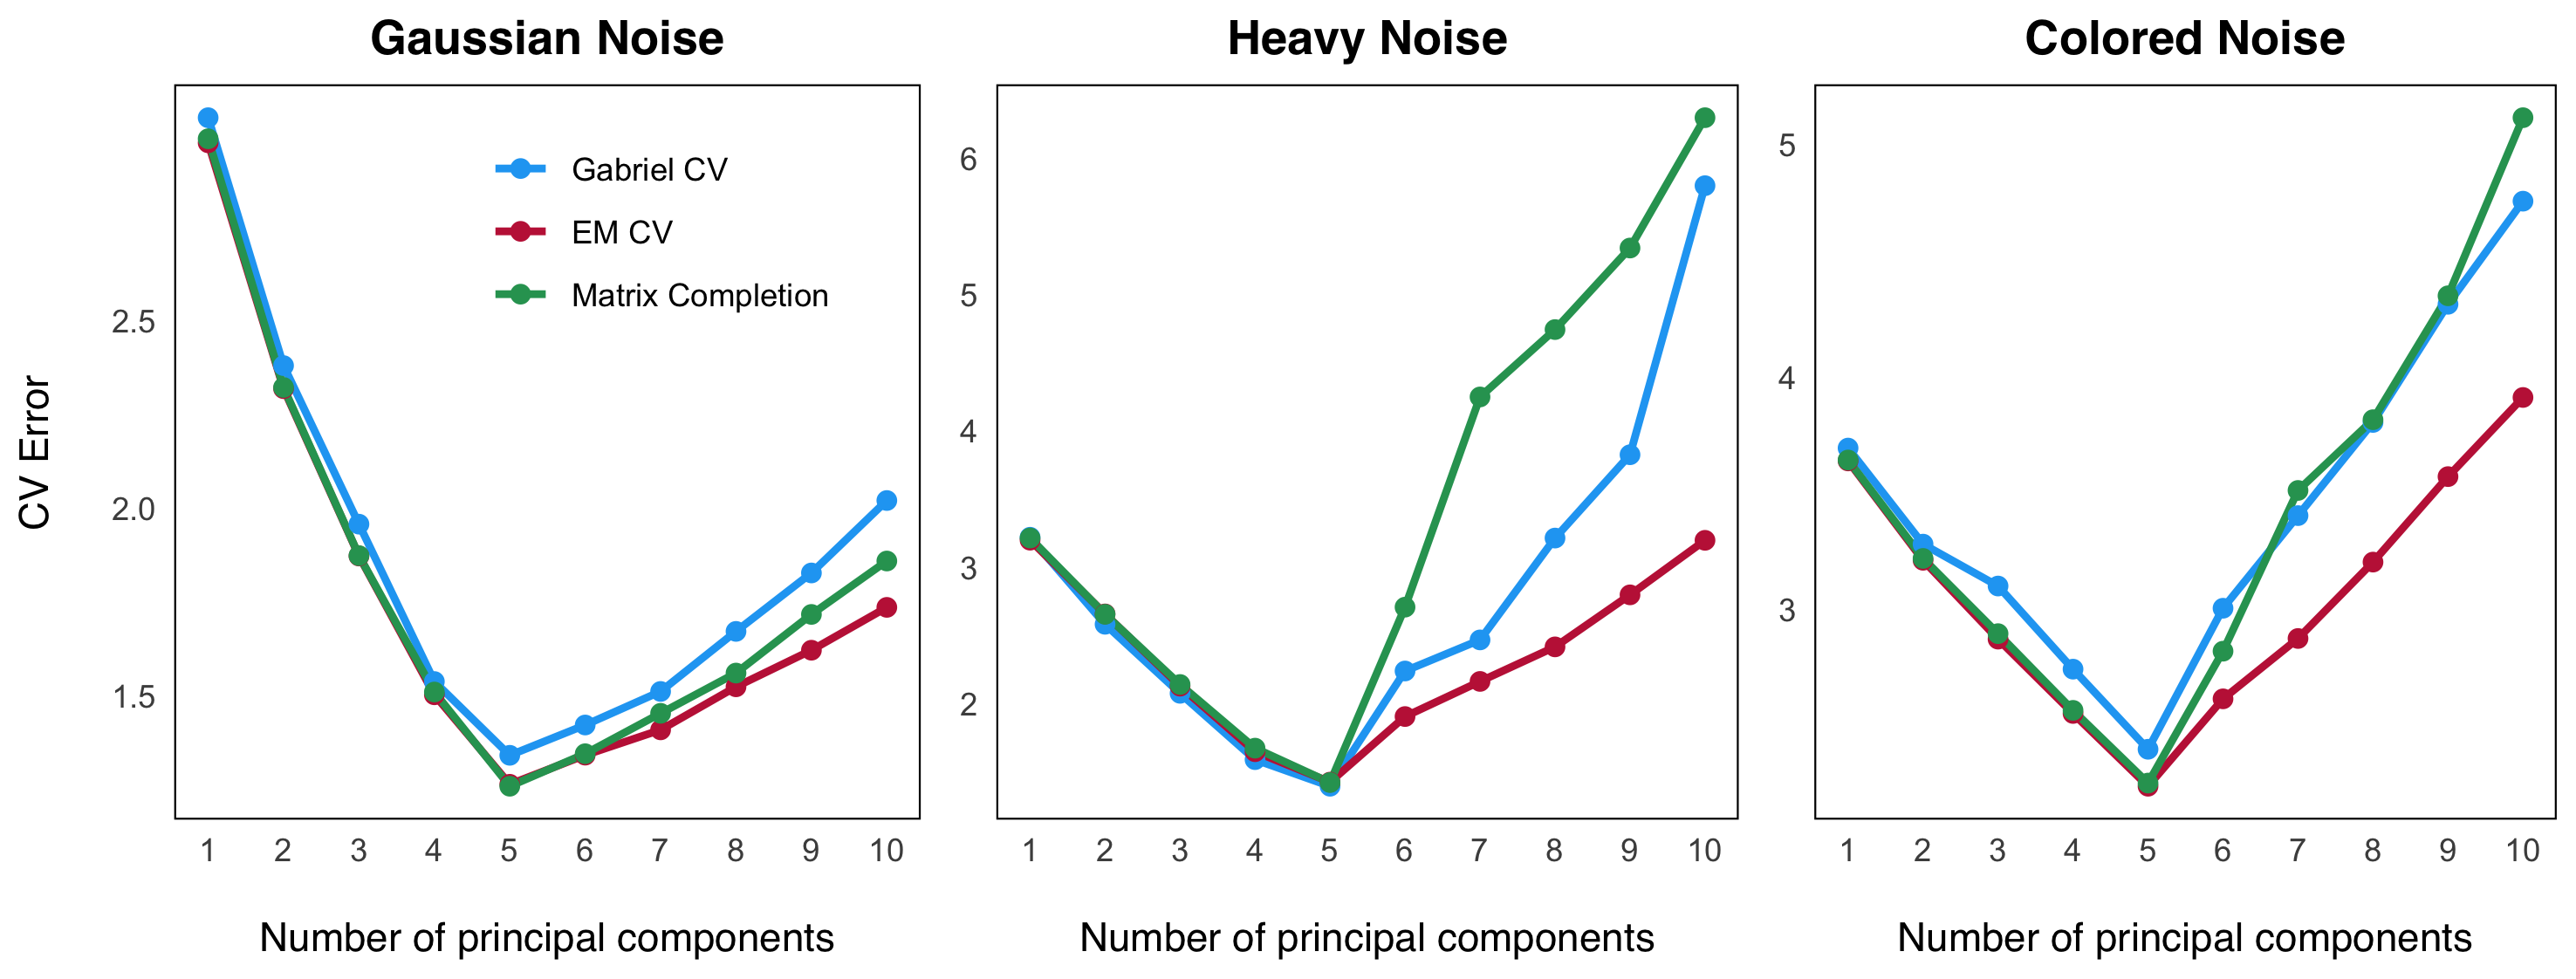
\includegraphics[width=\textwidth]{CVplots_highnoise.png}
    \caption{CV error of the three methods varying the noise, with low SNR}
    \label{fig:CV_error_high}
\end{figure}

As far as the computational cost is concerned, as it shows in Figure \ref{fig:Time}, Gabriel hold-out works 
much faster than both the other algorithms, with Matrix Completion working almost as 
fast for low ranks, and much slower for higher ranks. EM cross validation has a more 
constant execution time, more costly than Gabriel but definitely cheaper than Matrix 
Completion for high values of the principal subspace dimension. 


\begin{figure}[h!]
    \centering
    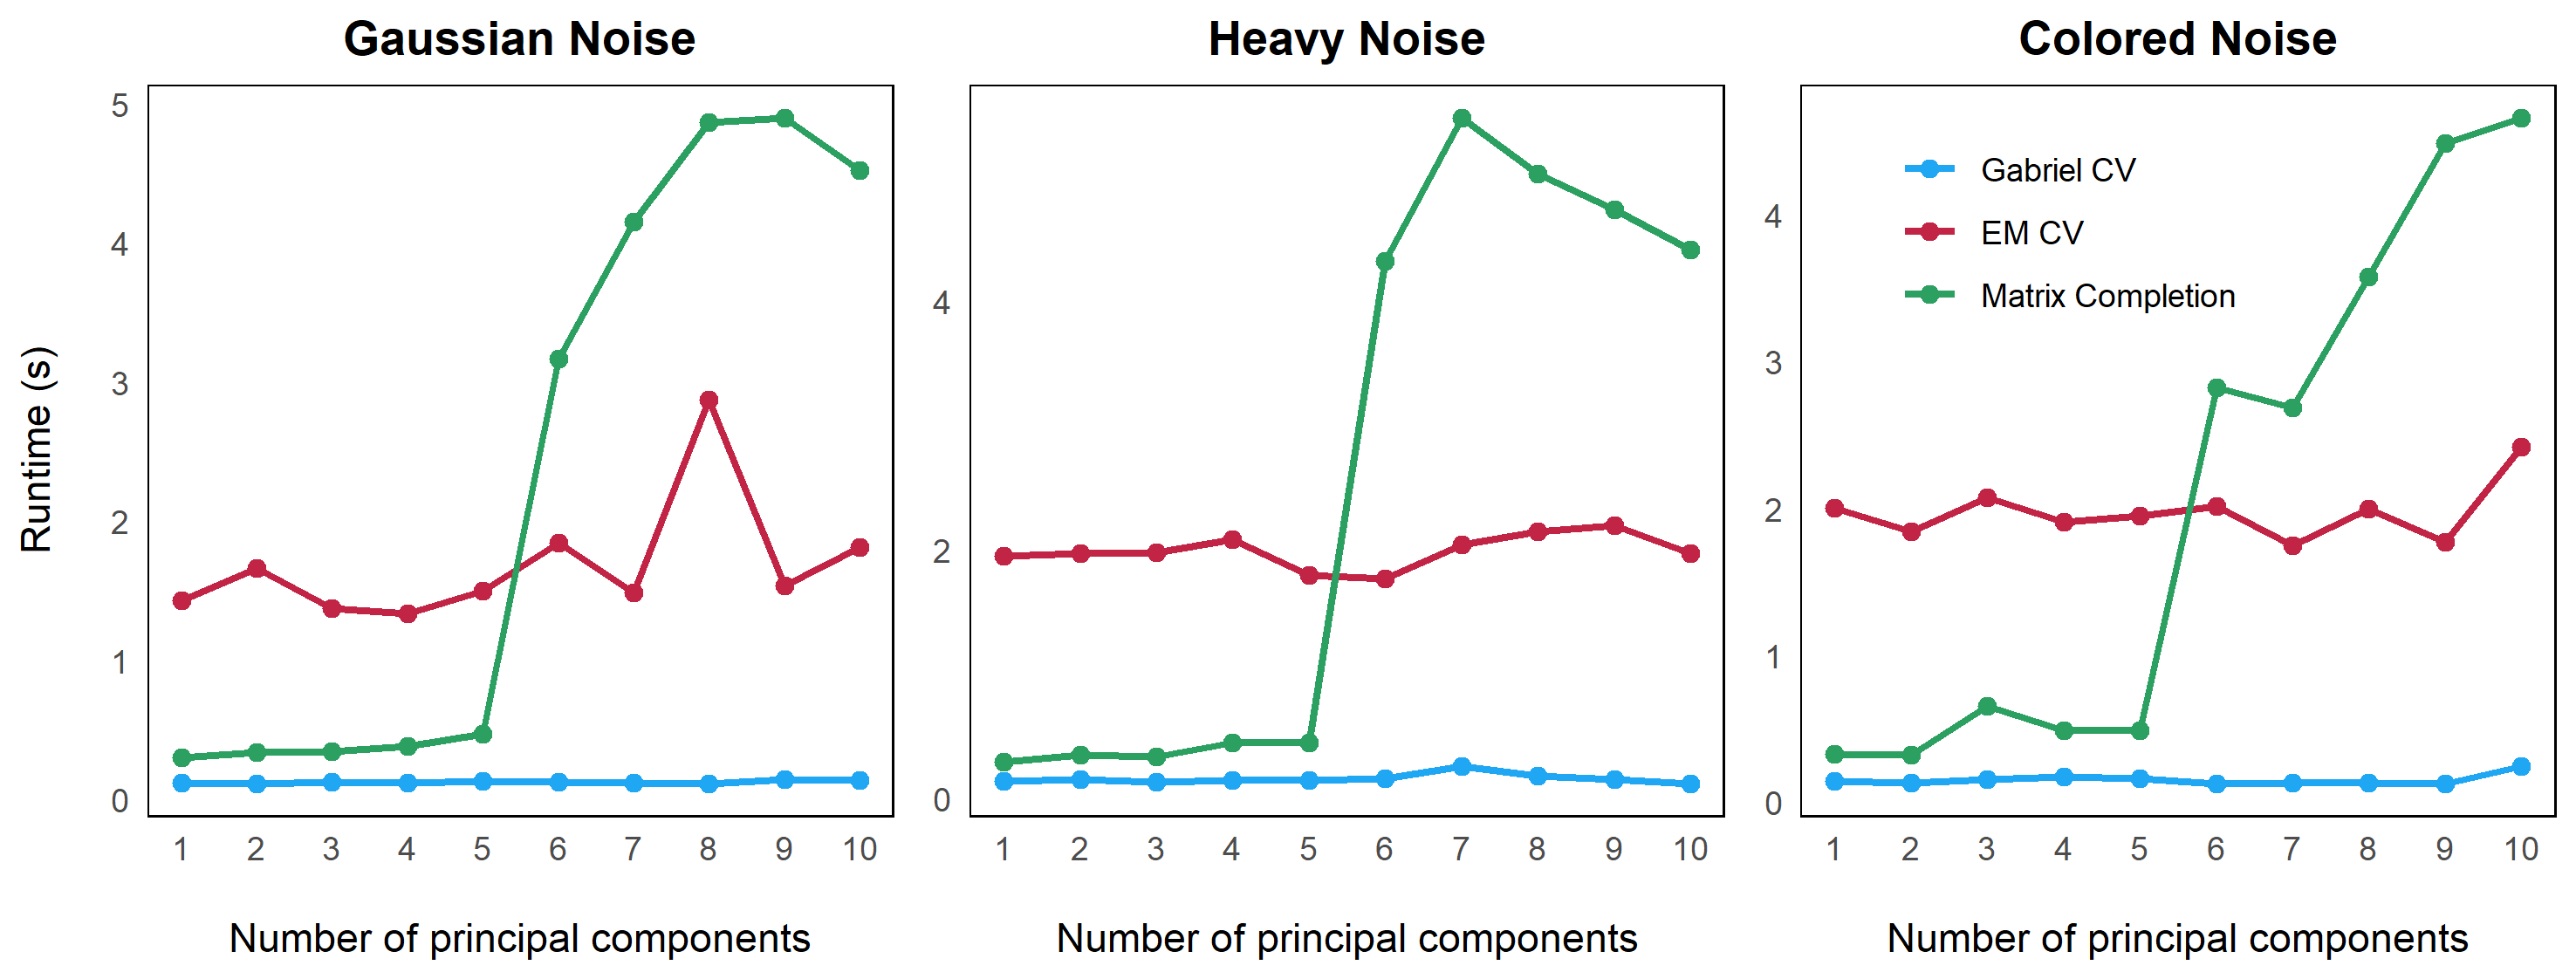
\includegraphics[width=\textwidth]{runtime.png}
    \caption{Runtime of the three methods varying the noise}
    \label{fig:Time}
\end{figure}

\subsubsection{Impact of the true rank}

A crucial aspect to investigate is the influence of the true rank, particularly its ratio to the total number
of features, on the accuracy of our three rank estimation methods. In our simulations, we set the true rank 
to 17, exceeding half of the total number of features.

Figure \ref{fig:Higher_rank} illustrates the performance of the methods under this scenario. While all 
methods successfully identified the correct rank in this specific instance, the EM cross-validation and 
Matrix Completion methods demonstrated more stable estimation behavior for higher ranks. In contrast, the 
Gabriel hold-out method exhibited a more erratic pattern, suggesting a potential sensitivity to the relative 
magnitude of the true rank compared to the total number of features.

This observation highlights the importance of considering the relative rank of the data when evaluating the performance of different dimensionality reduction techniques. Methods that exhibit stable behavior across a wide range of rank-to-feature ratios are likely to be more robust and reliable in practical applications.
\begin{figure}[h!]
    \centering
    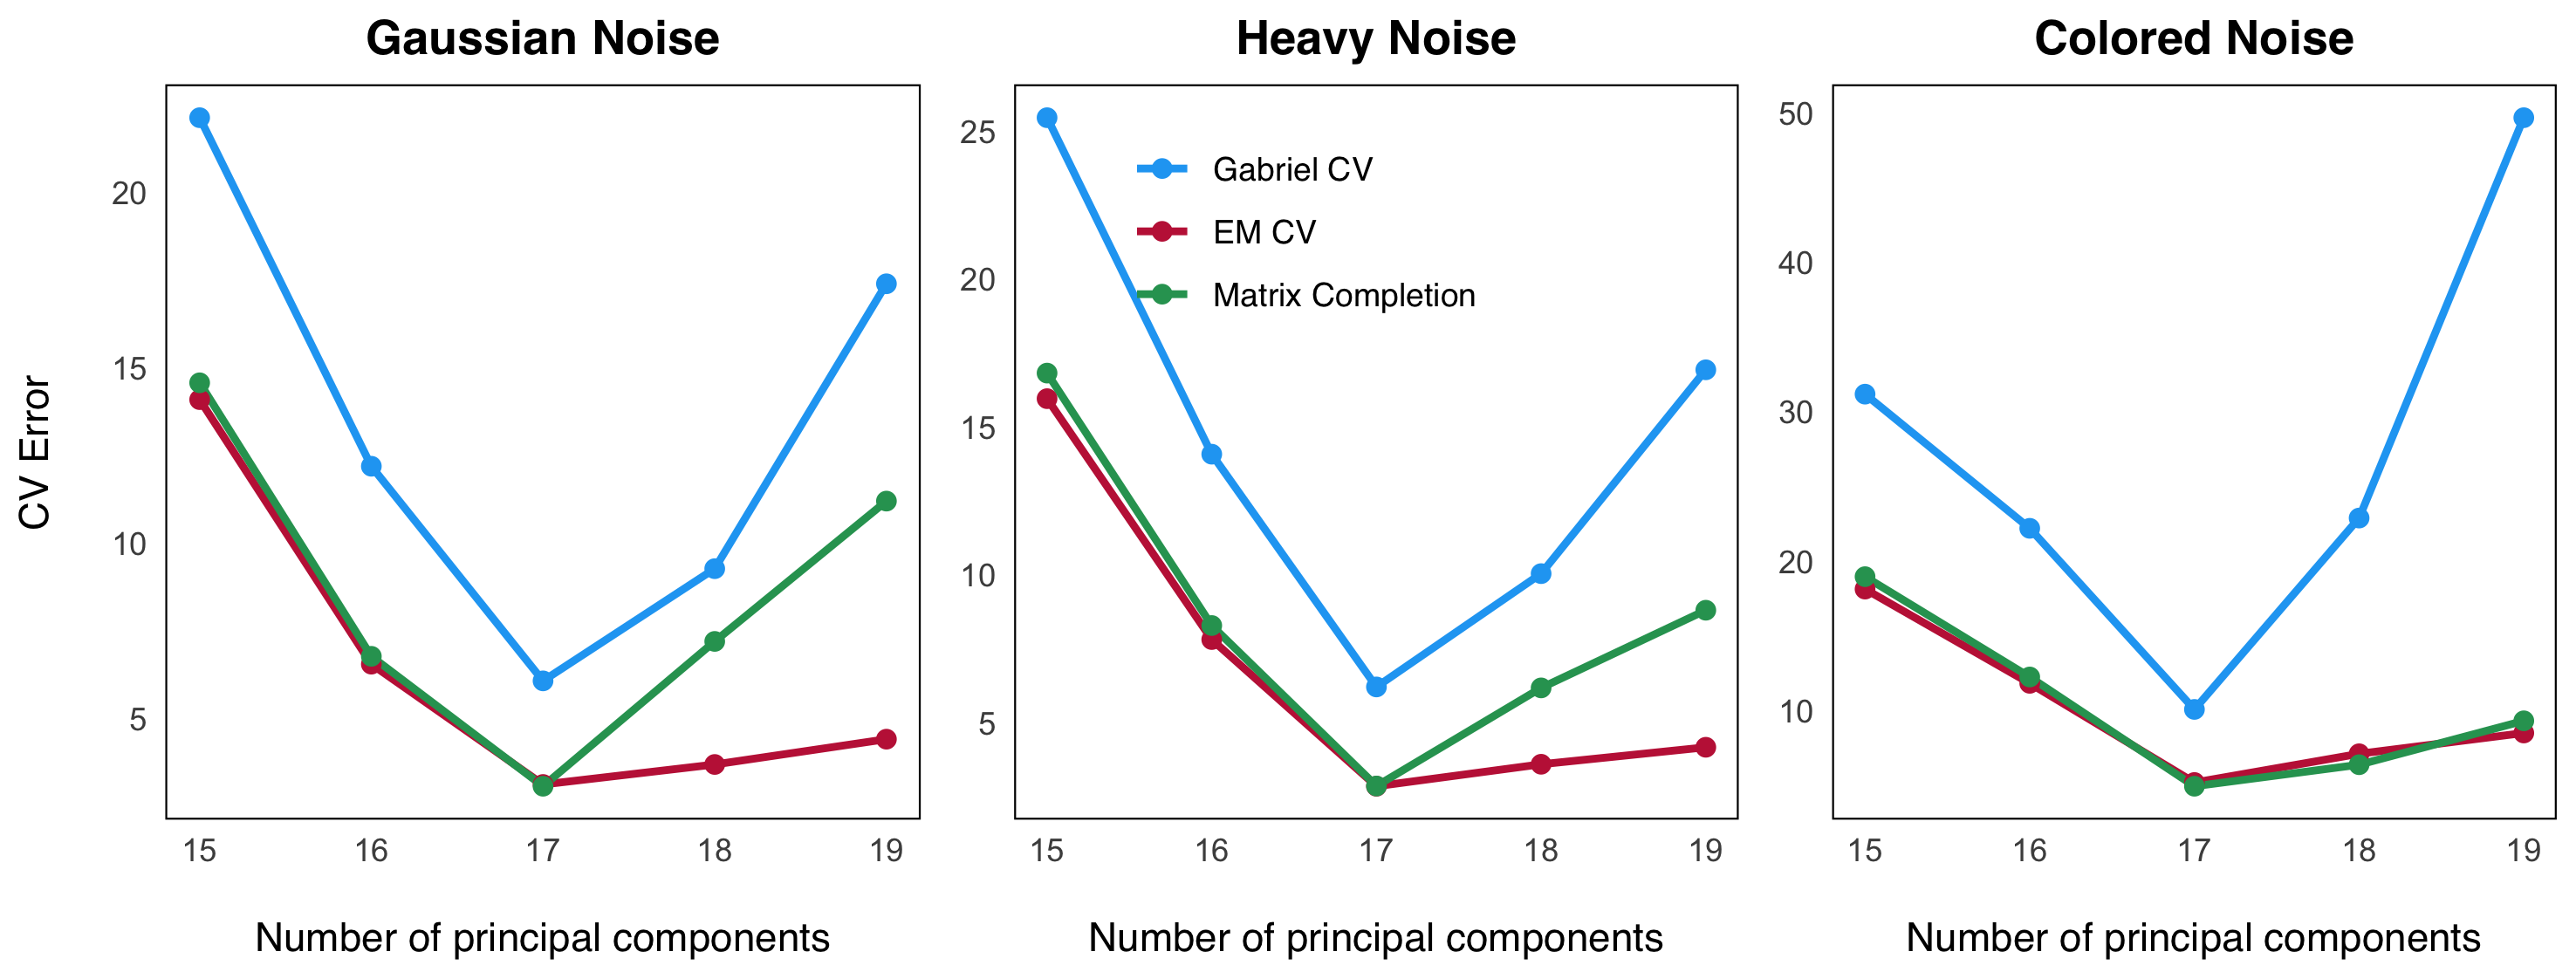
\includegraphics[width=\textwidth]{accuracy_high_rank.png}
    \caption{CV error of the three methods varying the noise with high rank}
    \label{fig:Higher_rank}
\end{figure}
\vspace{-5mm}
\subsubsection{Impact of the sample size}

Computational efficiency is a critical factor in practical applications, particularly when dealing with 
large datasets. Figure \ref{fig:Time_versus_n} clearly demonstrates a significant disparity in the 
computational cost of the three rank estimation methods.

The Gabriel hold-out method emerges as the most computationally efficient, exhibiting a nearly constant 
runtime with respect to the sample size. This characteristic makes it an attractive option for analyzing 
large datasets where computational speed is paramount.

The EM cross-validation method occupies an intermediate position. Its runtime increases linearly with the 
sample size, indicating a moderate computational cost.

In contrast, the Matrix Completion method demonstrates the highest computational cost. While its runtime 
also increases linearly with the sample size, the rate of increase is substantially higher compared to the 
other two methods. This significant computational overhead can render Matrix Completion impractical for very 
large datasets.

These findings underscore the importance of considering computational efficiency when selecting a rank 
estimation method. In scenarios where computational time is a critical constraint, the Gabriel hold-out 
method may be a viable alternative to more computationally intensive methods, particularly when dealing 
with large datasets. However, it is crucial to carefully weigh the trade-off between computational efficiency 
and the potential impact on the accuracy and reliability of the rank estimation.

\begin{figure}[h!]
    \centering
    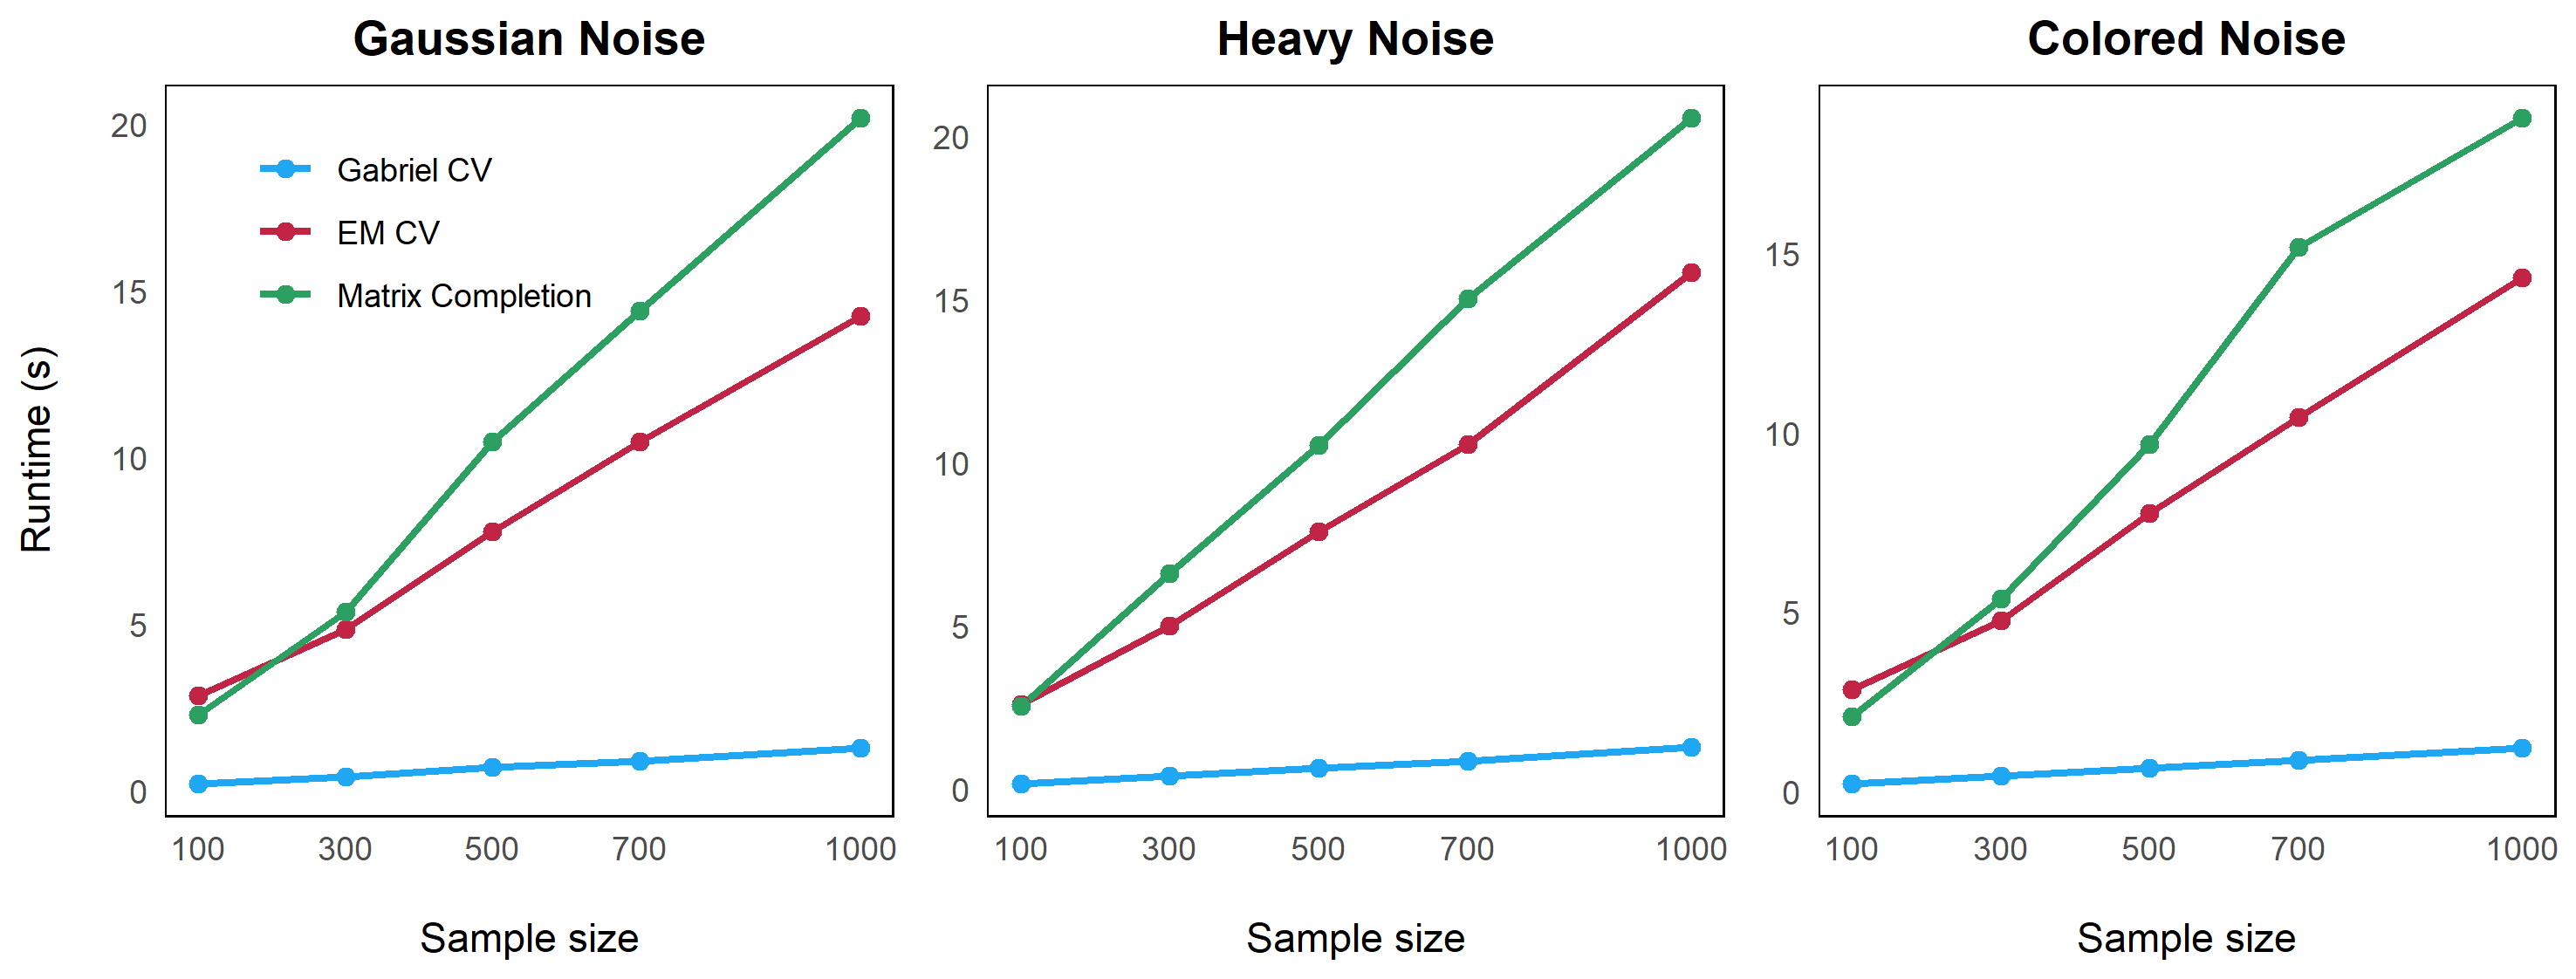
\includegraphics[width=\textwidth]{runtime_versus_n.png}
    \caption{Runtime of the three methods varying the sample size}
    \label{fig:Time_versus_n}
\end{figure}

\subsubsection{Accuracy of the methods on multiple runs}
To test the reliability of the three methods, we ran 100 simulations for each of the three methods, with the three types of noise, 
and we computed the frequency of times the correct rank was chosen. The sample size was reduced to $n=100$ to speed up the computation.
As shown in Figures \ref{fig:accuracy}, the EM method seems to be the most reliable overall, with the Gabriel hold-out being the least 
reliable. The MC method is in between the other two methods, with a performance that is more stable than the Gabriel 
hold-out, comparable to the EM method for Gaussian and colored noise, while being less reliable for heavy noise, almost as much 
as the Gabriel hold-out.

\begin{figure}[H]
    \centering
    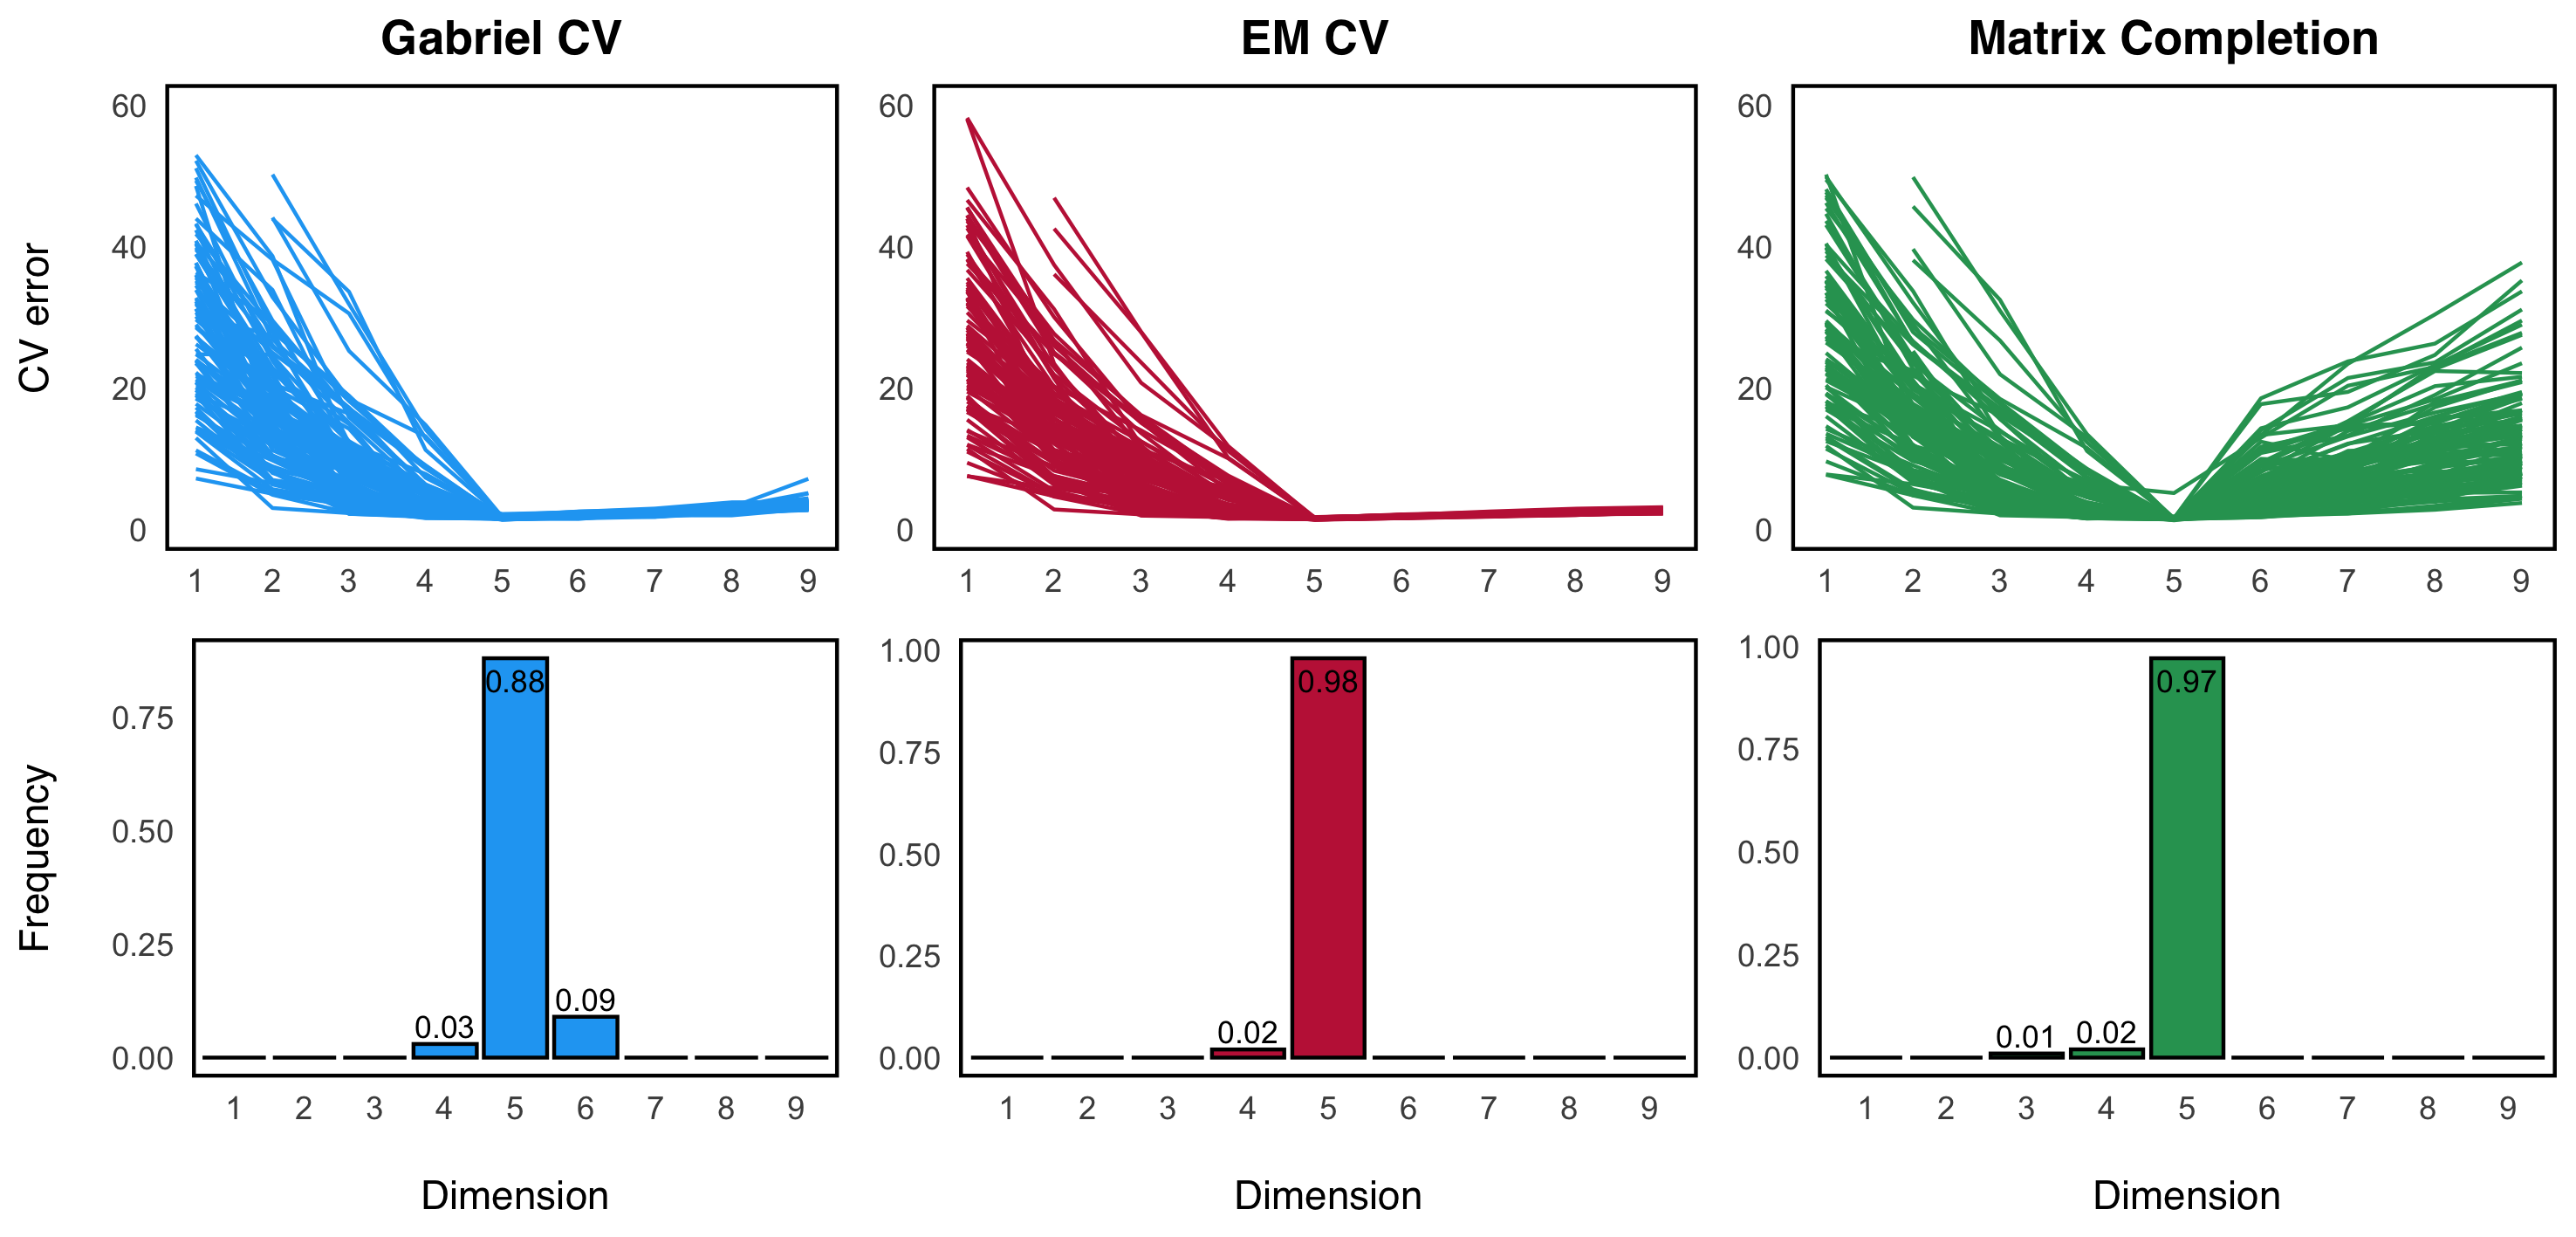
\includegraphics[width=\textwidth]{100gaussian.png}
\end{figure}

\begin{figure}[H]
    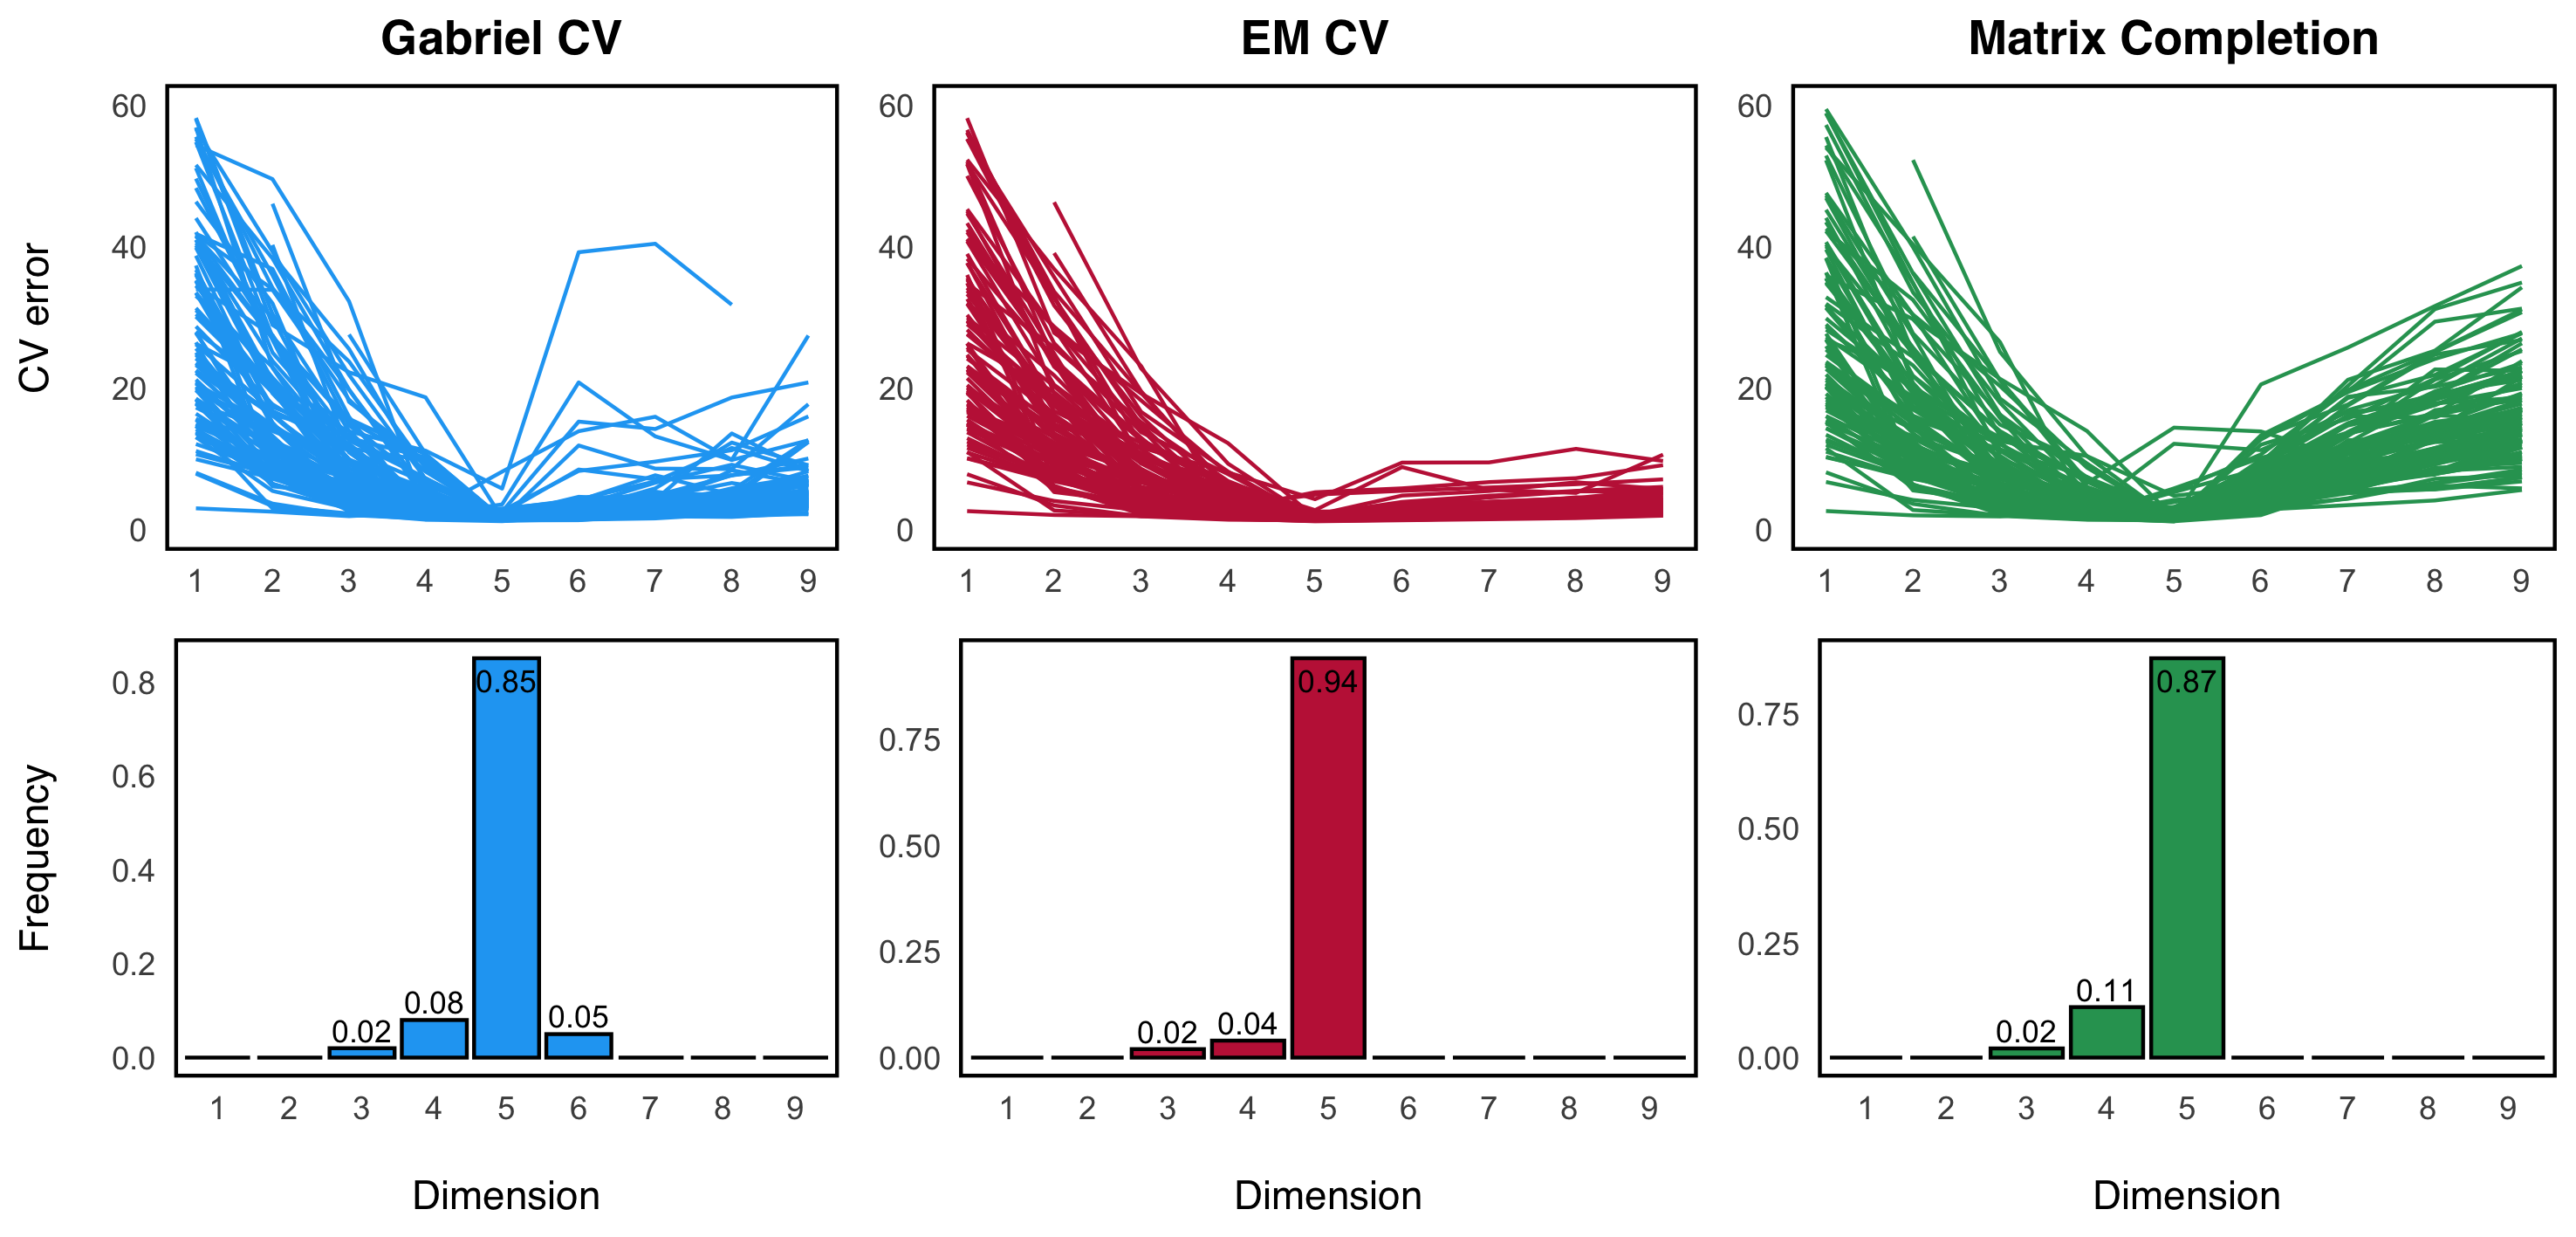
\includegraphics[width=\textwidth]{100heavy.png}
    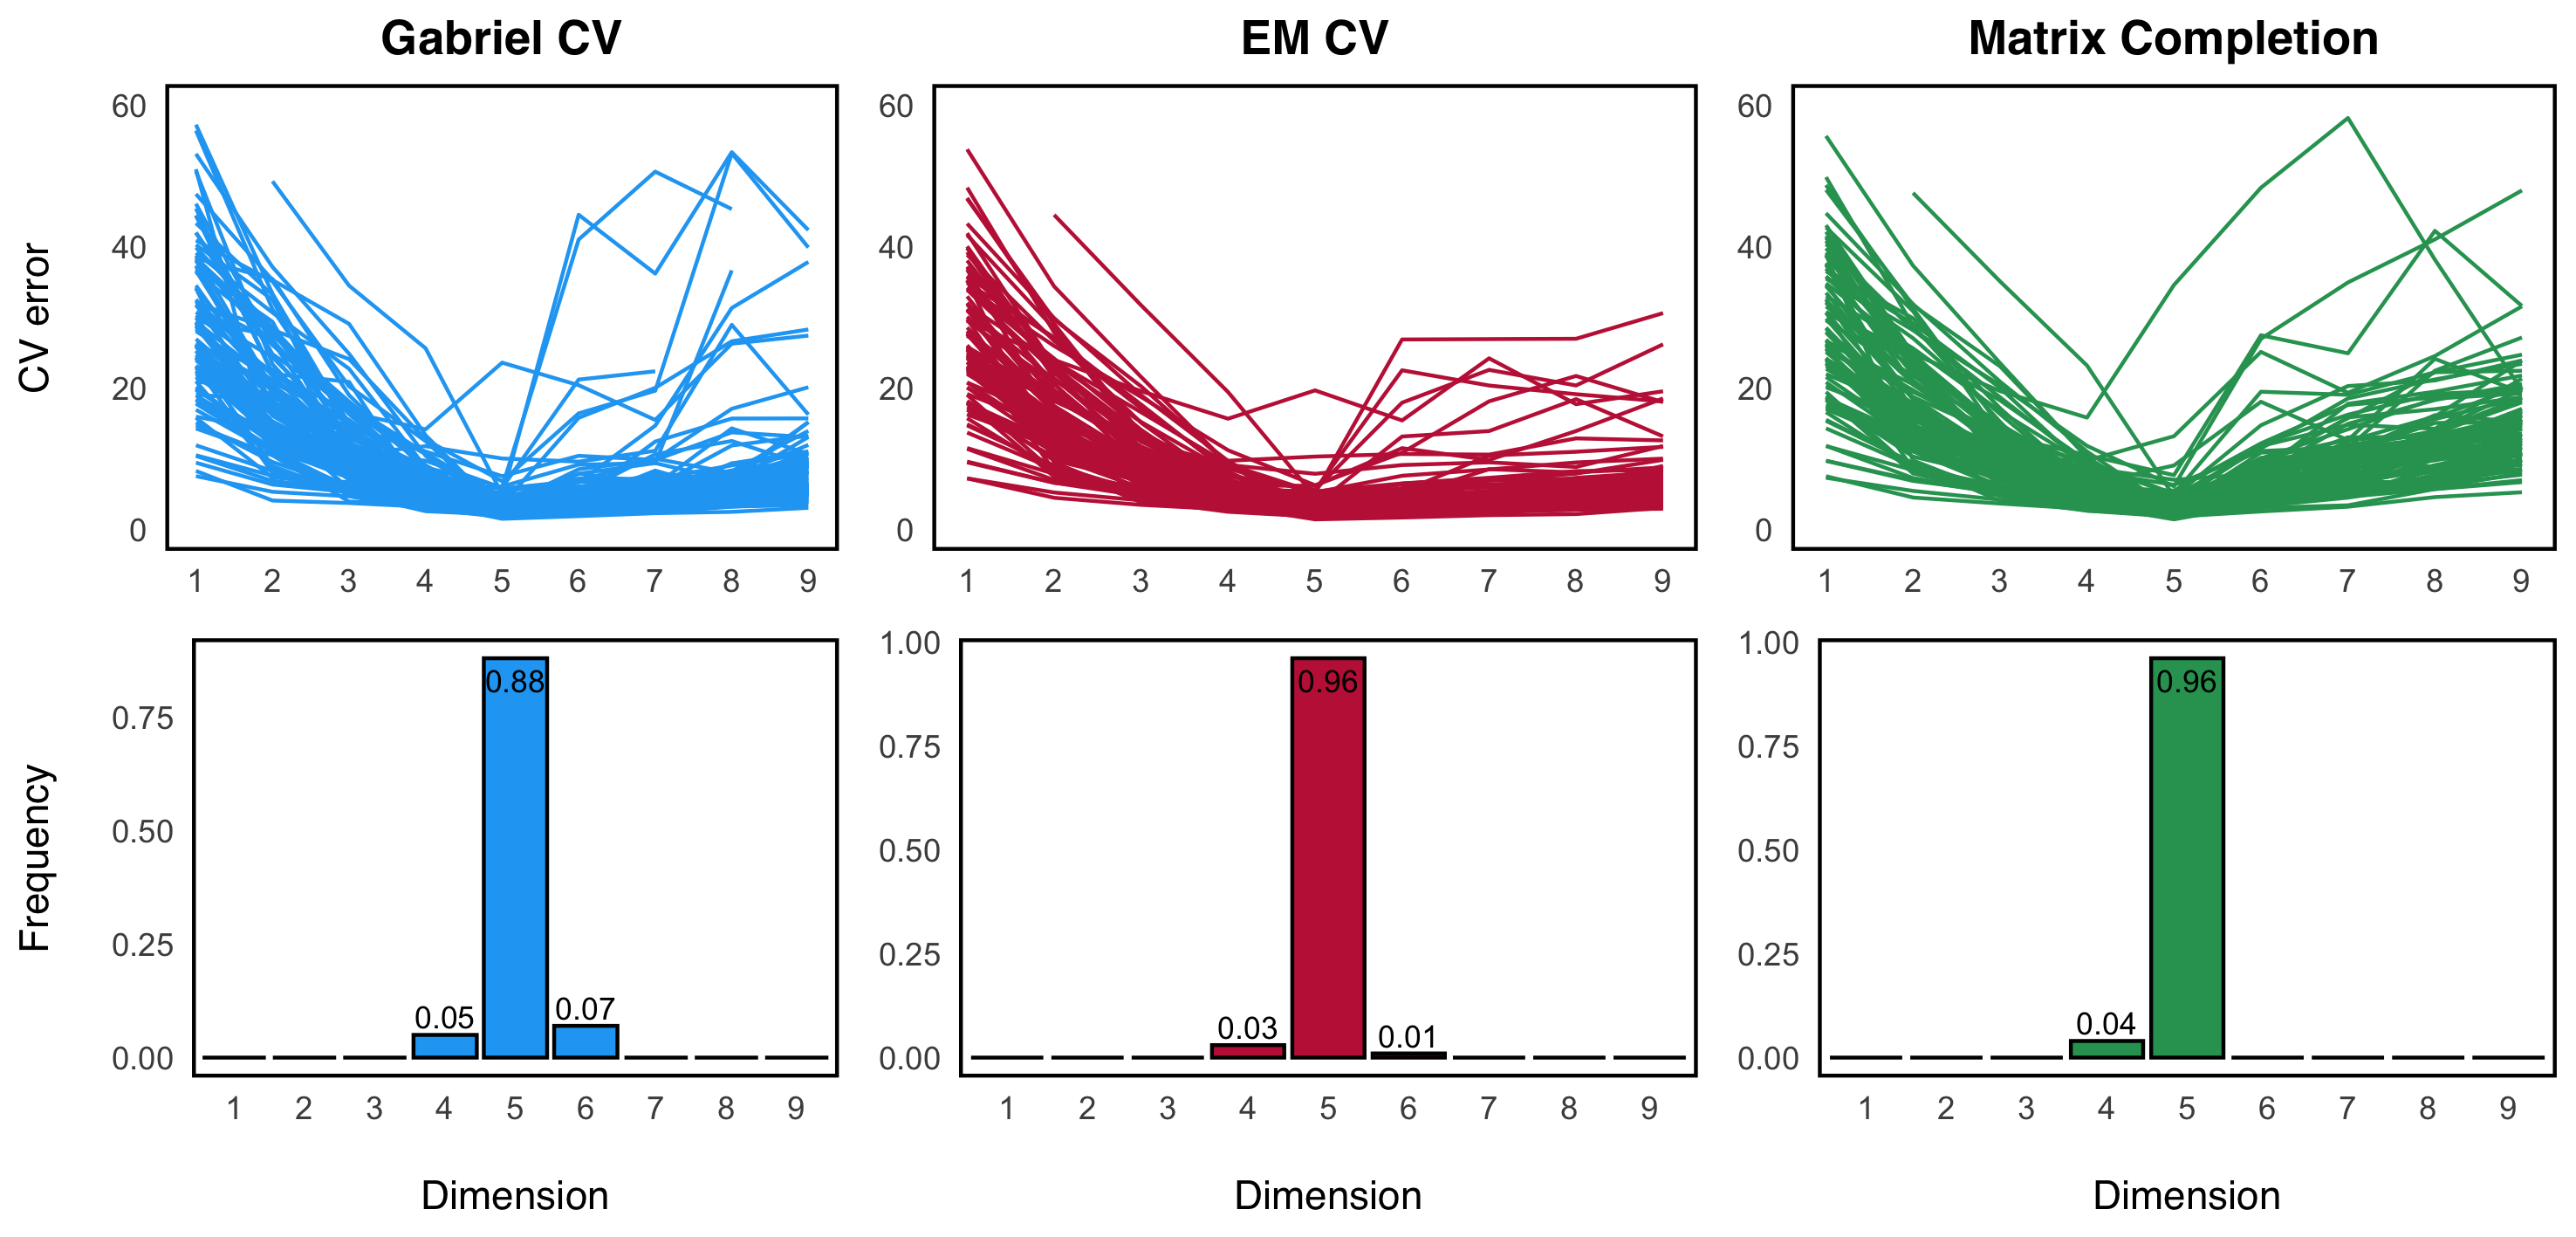
\includegraphics[width=\textwidth]{100colored.png}
    \caption{Accuracy of the three methods. From the top to the bottom we applied: Gaussian noise, Heavy noise, Colored noise}
    \label{fig:accuracy}
\end{figure}



\subsection{Discussion of the results on real data}
Our analysis of the Aphids dataset, a well-studied benchmark in the literature, provides a valuable case 
study for evaluating the performance of our proposed rank estimation methods. Previous studies have yielded 
conflicting results regarding the intrinsic dimensionality of this dataset. Krzanowski (1987) \cite{Krzanowski} 
and Diana (2002) \cite{Diana} employed advanced techniques and concluded that the intrinsic dimensionality is 
4, while Jeffers (1967) \cite{Jeffers}, using more traditional approaches, estimated it to be 2.

Interestingly, all three of our proposed methods consistently indicated an 
intrinsic dimensionality of 2 for the Aphids dataset (see Figure \ref{fig:aphids}), aligning with Jeffers' earlier findings. This apparent 
discrepancy with the more recent studies warrants careful consideration.

\begin{figure}[h!]
    \centering
    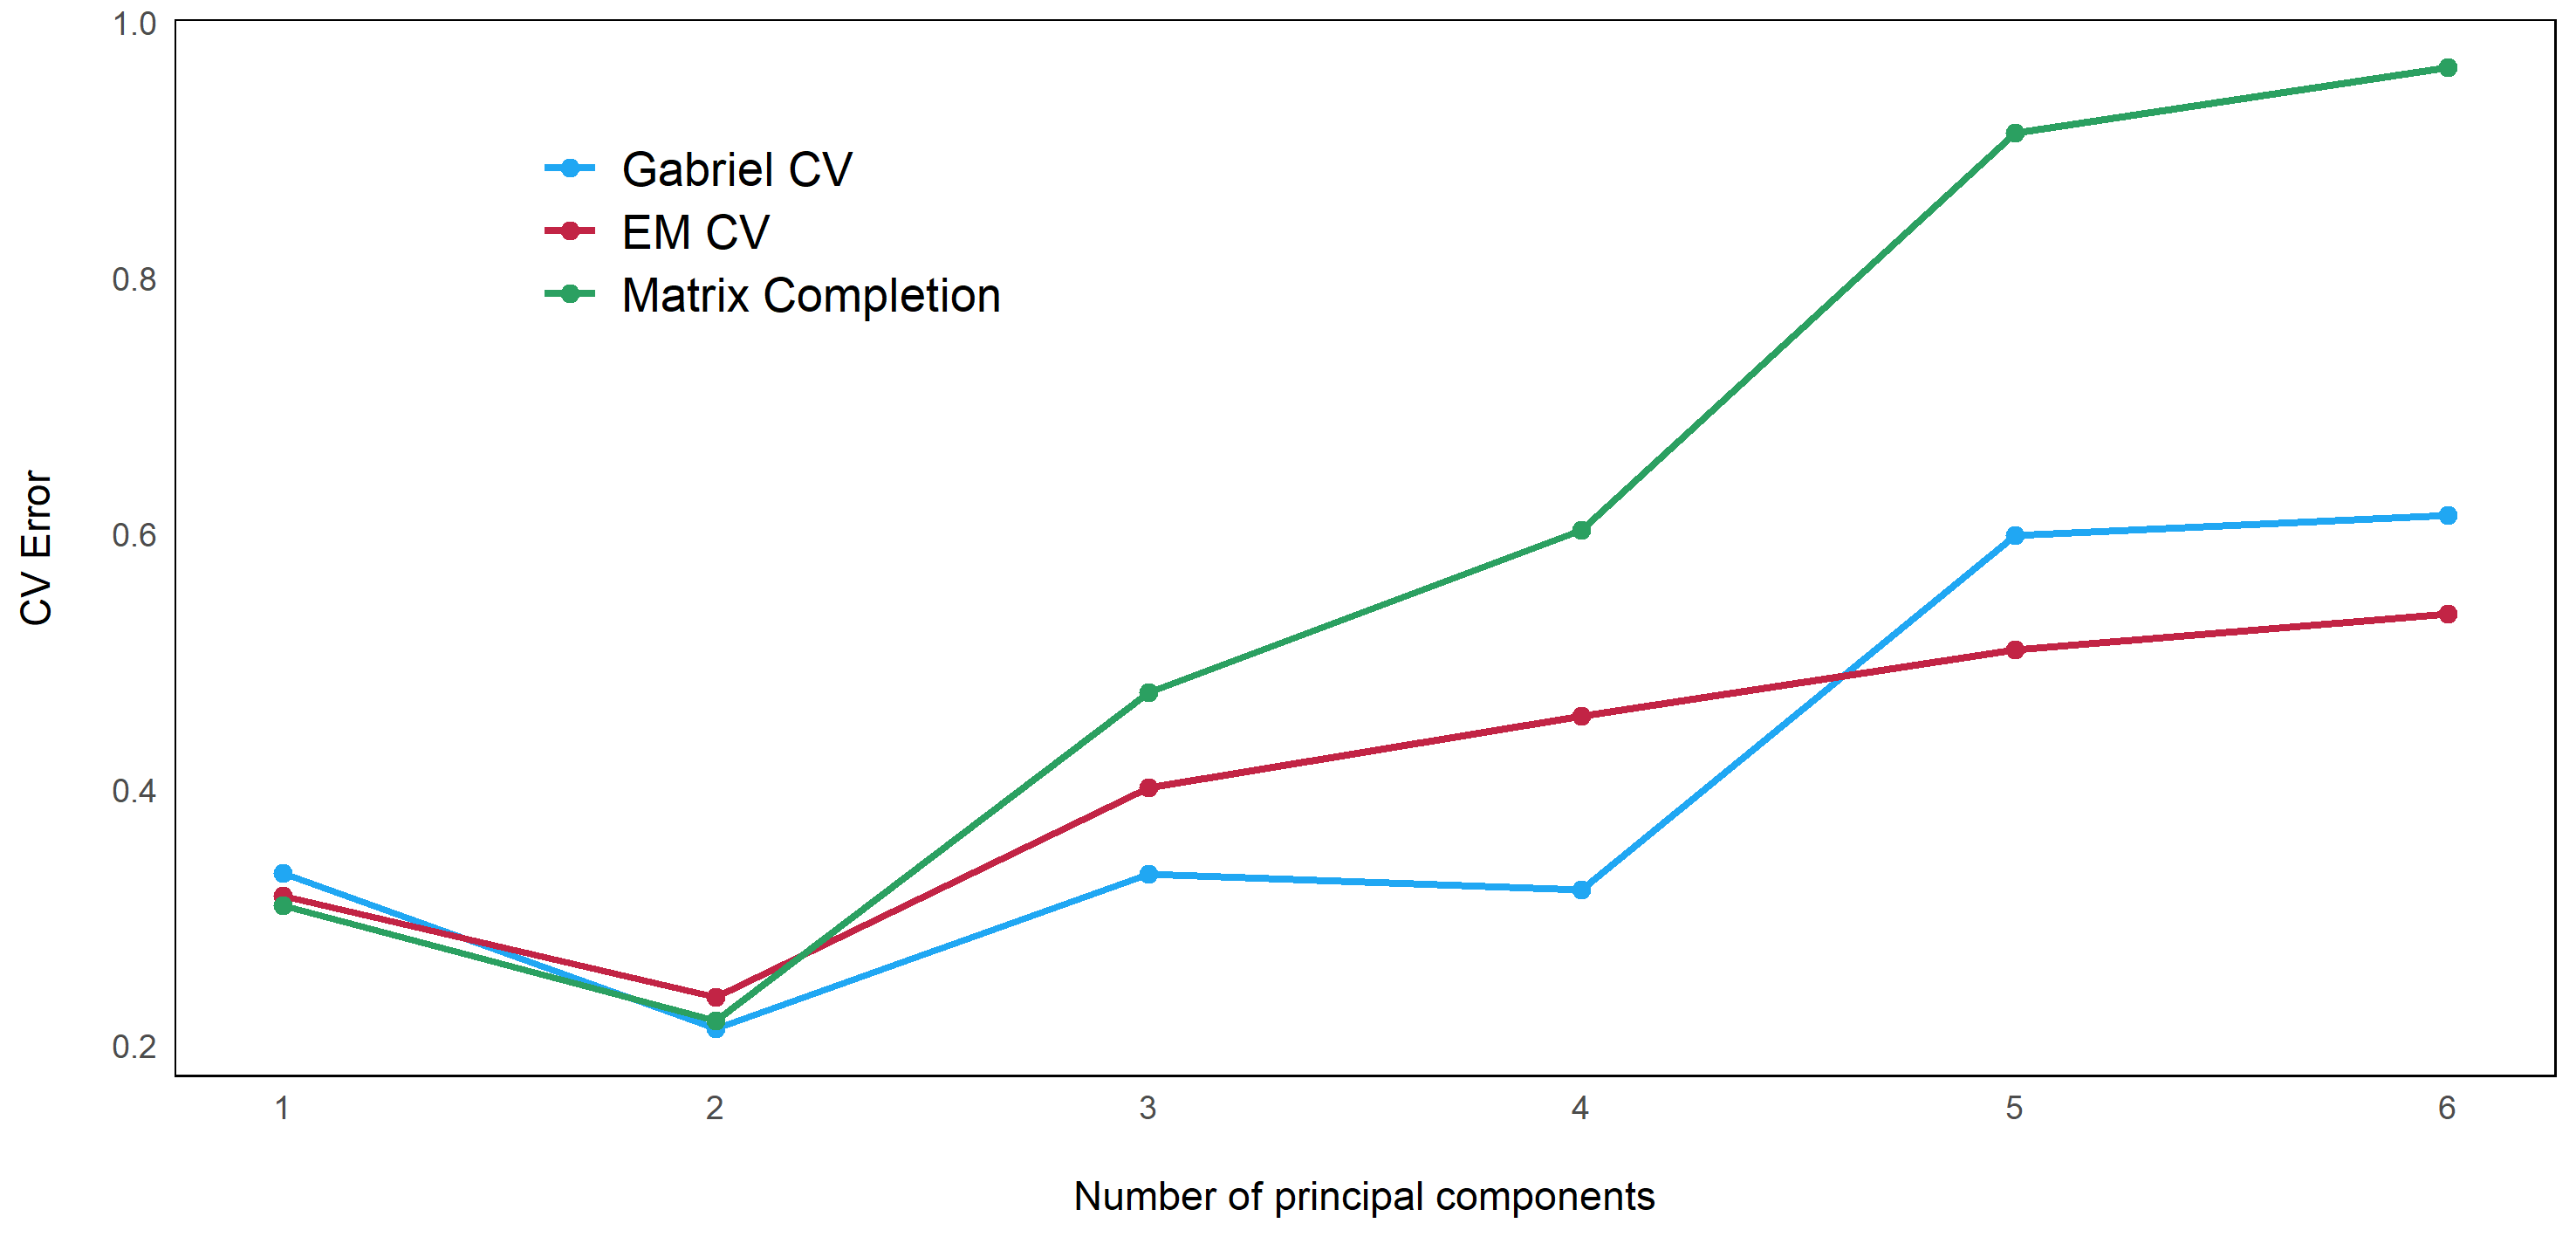
\includegraphics[width=0.8\textwidth]{aphids.png}
    \caption{CV on the Aphids dataset}
    \label{fig:aphids}
\end{figure}

Several factors may contribute to this outcome. Firstly, the Aphids dataset is relatively small, comprising 
only 40 observations. The limited sample size can significantly impact the accuracy of dimensionality 
estimation, particularly for methods that rely on strong assumptions about the data distribution.
Secondly, the EM and Gabriel hold-out methods are inherently based on the assumption of Gaussianity in the 
data. However, our tests using Mardia's and Royston's tests unequivocally rejected the hypothesis of 
Gaussianity for the Aphids dataset. This violation of the underlying assumption likely contributed to the 
suboptimal performance of these methods.

Even the Matrix Completion method, which does not explicitly rely on Gaussianity, exhibited subpar performance 
on this dataset. This suggests that the small sample size may have hindered accurate estimation of missing 
entries, a crucial step in the Matrix Completion process.

In contrast, our analysis of the air pollution dataset yielded more promising results. Dray (2008) \cite{Dray} 
previously estimated the intrinsic dimensionality of this dataset to be 3. In our evaluation, the Matrix 
Completion method emerged as the most reliable, accurately identifying the correct number of components. 
The other two methods, EM and Gabriel hold-out, failed to correctly estimate the true dimensionality.

\begin{figure}[h!]
    \centering
    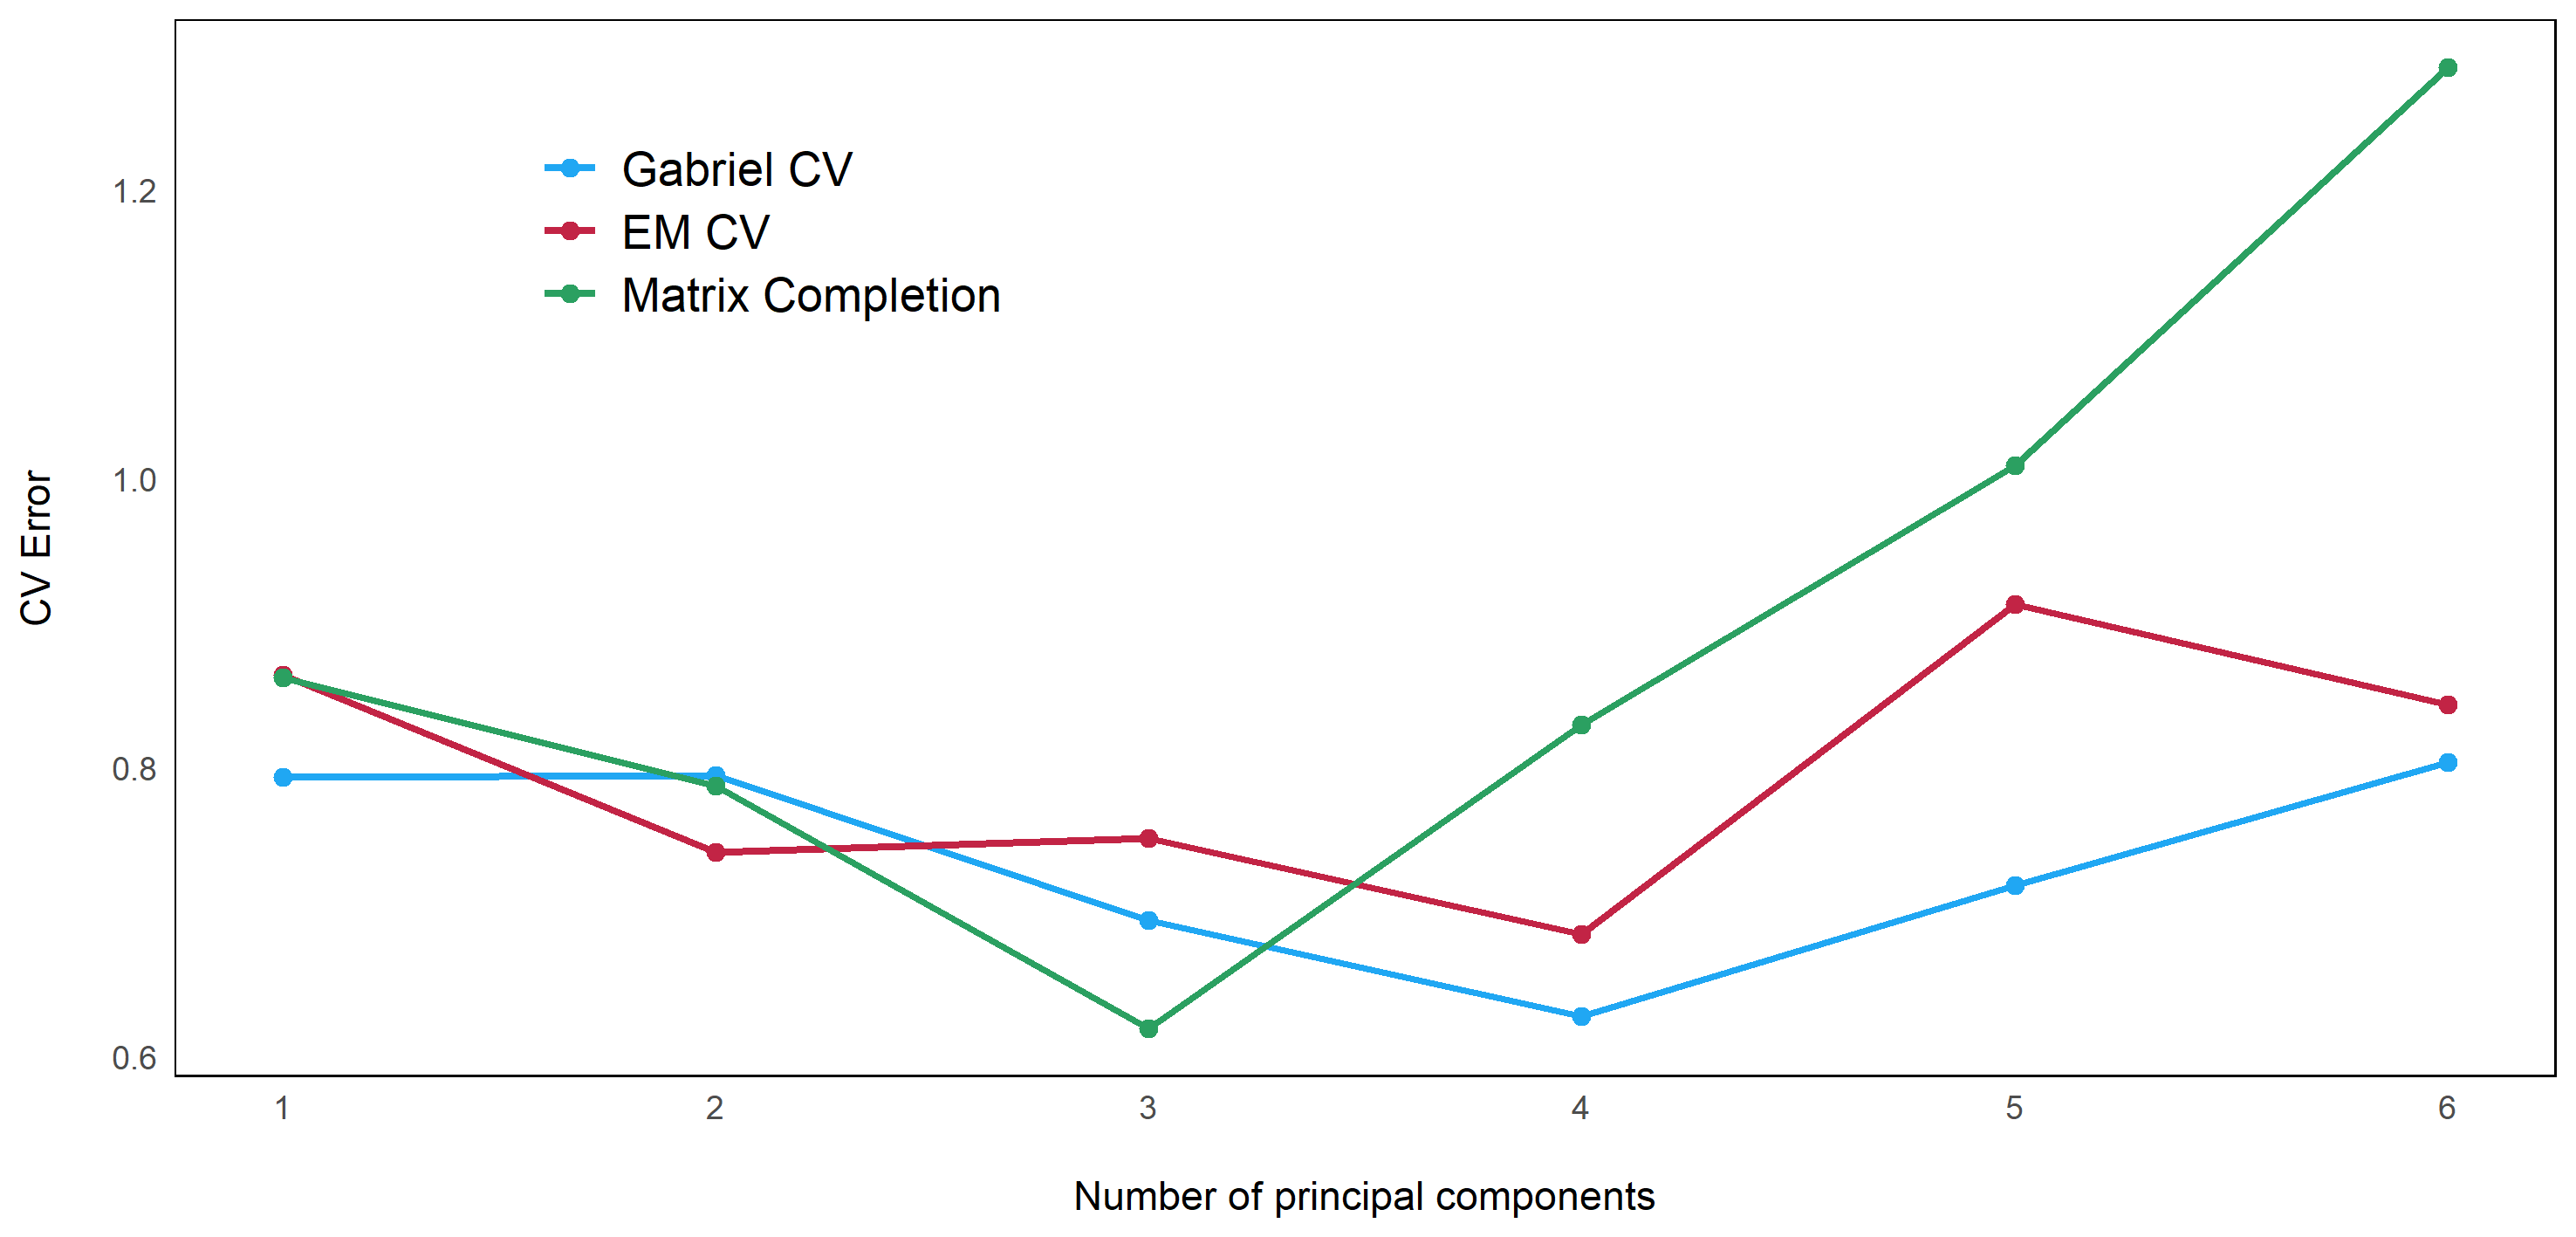
\includegraphics[width=0.75\textwidth]{pollution.png}
    \caption{CV on the Air Pollution dataset}
    \label{fig:pollution}
\end{figure}
These findings underscore the importance of considering the specific characteristics of the dataset, 
including sample size and underlying data distribution, when selecting and applying dimensionality estimation 
methods. While our proposed methods demonstrated varying degrees of success across different datasets, the 
results highlight the challenges and potential limitations associated with dimensionality estimation in 
real-world scenarios.

\section{Conclusions}
In this study, we explored three cross-validation techniques—Gabriel Hold-Out, EM, 
and Matrix Completion—for determining the optimal number of components in Principal Component Analysis. 
Through simulations on synthetic datasets, we highlighted the strengths and weaknesses of each method, 
emphasizing the trade-offs between computational efficiency, stability, and accuracy. Gabriel Hold-Out 
emerged as the most computationally efficient, while EM demonstrated robustness across various noise types. 
Matrix Completion, despite its higher computational cost, demonstrated reliable performance in scenarios characterized
 by complex noise structures. Additionally, in cases where the noise has a limited impact, this method provides a more 
 decisive selection of the optimal rank.\\
When applied to real-world datasets, the methods revealed their limitations, particularly concerning sample size 
and assumptions about data distribution. For example, the small sample size and lack of Gaussianity in the Aphids 
dataset posed challenges for all three methods, while the air pollution dataset underscored the effectiveness of Matrix Completion.\\
These findings illustrate that the choice of method should consider dataset-specific characteristics. Future research could 
focus on refining these techniques to enhance their applicability to diverse real-world contexts, improving their performance 
under varying conditions.


\begin{thebibliography}{9}
    \bibitem{perry} 
    Perry, P.O. (2009). 
    \href{https://citeseerx.ist.psu.edu/document?repid=rep1&type=pdf&doi=0a2508a9fd89513ddf1c227274c8192993520692}{Cross-Validation for Unsupervised Learning}. 
    Stanford University.

    \bibitem{Jeffers}
    Jeffers, J.N.R. (1967).
    \href{https://www.jstor.org/stable/2985919}{Applied Statistics}.
    Two Case Studies in the Application of Principal Component Analysis

    \bibitem{Krzanowski}
    Krzanowski, W.J. (1987).
    \href{https://www.tandfonline.com/doi/abs/10.1080/03610928708829385}{Applied Statistics}.
    Selection of Variables to Preserve Multivariate Data Structure, Using Principal Components 
    
    \bibitem{Diana}
    Diana, G.; Tommasi, C. (2002).
    \href{https://link.springer.com/article/10.1007/BF02511446}{Computational Statistics \& Data Analysis}.
    Cross-validation methods in principal component analysis: A comparison 

    \bibitem{Dray}
    Dray, S. (2008).
    \href{https://www.sciencedirect.com/science/article/pii/S0167947307002939}{Computational Statistics \& Data Analysis}.
    On the number of principal components: A test of dimensionality based on measurements of similarity between matrices

\end{thebibliography}

\end{document}